\documentclass[11pt,a4paper]{article}
\usepackage[T1]{fontenc}
\usepackage[utf8]{inputenc}
\usepackage{lmodern}
\usepackage[british]{babel}
\usepackage[margin=24mm,headheight=15pt]{geometry}
\usepackage{amsmath,amssymb,graphicx,booktabs,longtable,array,tabularx}
\usepackage{float,caption,xcolor,enumitem,microtype,fancyhdr}
\usepackage{etoolbox}
% Compatibility fix for longtable v4.24 (latex3/latex2e issue 1907).
% Upstream v4.25 uses finite shrink in these two output-routine skips.
% On newer versions the patterns do not occur and this is a no-op.
\makeatletter
\patchcmd{\LT@output}{\vss}{\vskip\z@\@plus1fil\@minus\normalbaselineskip}{}{}
\patchcmd{\LT@output}{\vss}{\vskip\z@\@plus1fil\@minus\normalbaselineskip}{}{}
\makeatother
\usepackage[numbers,sort&compress]{natbib}
\usepackage{xurl}
\usepackage[unicode,colorlinks=true,linkcolor=teal!60!black,citecolor=teal!60!black,urlcolor=teal!60!black]{hyperref}
\definecolor{ink}{HTML}{183C50}
\definecolor{accent}{HTML}{155E75}
\setlength{\parskip}{4pt}
\setlength{\parindent}{0pt}
\setlength{\emergencystretch}{2em}
\setlength{\tabcolsep}{5pt}
\renewcommand{\arraystretch}{1.16}
\captionsetup{font=small,labelfont=bf,skip=8pt}
\setlist{nosep,leftmargin=*}
\pagestyle{fancy}
\fancyhf{}
\fancyhead[L]{\small\textcolor{ink}{Reactive seabed mat: scientific software report}}
\fancyhead[R]{\small TalentON 2026}
\fancyfoot[C]{\thepage}
\renewcommand{\headrulewidth}{0.3pt}
\hypersetup{pdftitle={A Selective Reactive Seabed Mat: Scientific Basis, Model Assumptions and Demonstrator Results},pdfsubject={Documented report of the TalentON 2026 software repository},pdfkeywords={keratin, reactive cap, seabed, lead, mercury, copper, finite volume, monitoring, maintenance}}
\newcommand{\sourcecode}[1]{\texttt{\small\detokenize{#1}}}
\newcommand{\figpage}[3]{\begin{figure}[p]\centering\includegraphics[width=\linewidth,height=.78\textheight,keepaspectratio]{figures/#1.pdf}\caption{#2}\label{#3}\end{figure}}
\newcommand{\sourceRevision}{f3bbcf7d7d4ae755edb0d2d49480ba2799fdadc3}

\begin{document}
\hypersetup{pageanchor=false}
\begin{titlepage}
\vspace*{12mm}
{\large\textcolor{accent}{TALENTON 2026\quad /\quad TECHNICAL MANUSCRIPT}}\par
\vspace{14mm}
{\Huge\bfseries\textcolor{ink}{A Selective Reactive\\[4pt] Seabed Mat}}\par
\vspace{7mm}
{\Large Scientific basis, model assumptions\\ and demonstrator results}\par
\vspace{9mm}
{\large Keratin media, Pb--Hg--Cu transport, monitoring\\ and maintenance in an offline research demonstrator}\par
\vspace{13mm}
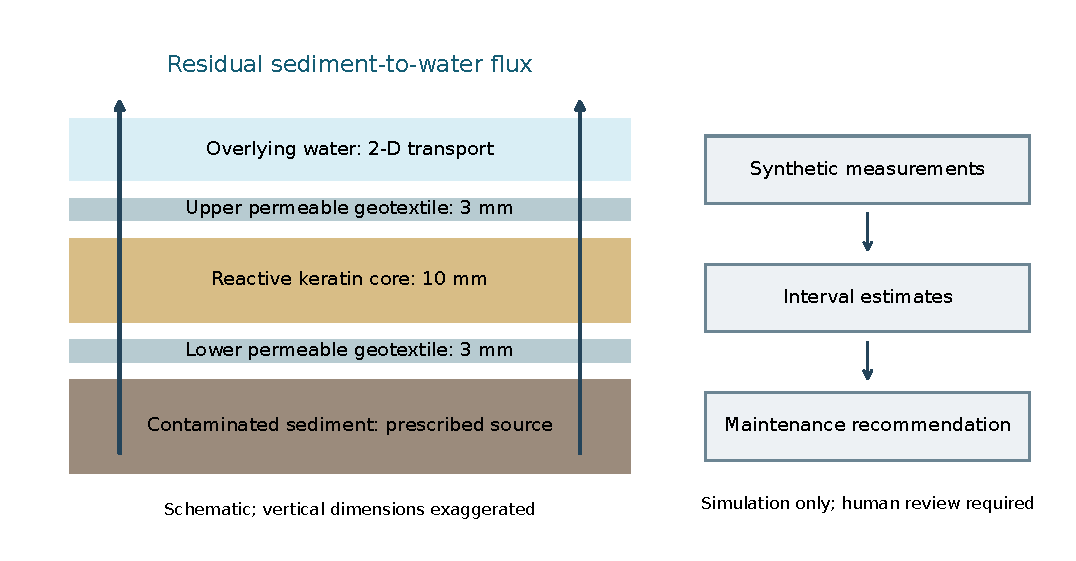
\includegraphics[width=\linewidth]{figures/concept.pdf}
\vfill
\begin{minipage}{\linewidth}\small
Prepared from the inspected \texttt{reactive-seabed-mat-demo} software snapshot.\\
Scientific source revision: \texttt{\sourceRevision}.\\
Report date: 9 September 2026.\quad Software version: 0.2.0.\\[5pt]
\textbf{Evidence status:} synthetic computational demonstration. The manuscript distinguishes external measurements, explicit assumptions, regenerated outputs and independent numerical checks. The proposed keratin mat has no field validation in the inspected evidence.
\end{minipage}
\end{titlepage}
\pagenumbering{roman}
\hypersetup{pageanchor=true}
\section*{Abstract}
\addcontentsline{toc}{section}{Abstract}
A thin modular reactive mat is investigated as a means of reducing contaminant flux from a contaminated sediment source. The software combines one-dimensional reactive transport in a keratin core, geotextile resistance, independent tile-condition variables, two-dimensional coastal transport, synthetic observations, interval estimates and maintenance recommendations. This report documents all operating assumptions, the supplied keratin literature, six regenerated scenarios, three servicing policies and independent numerical checks.

In the six-year baseline, whole-hotspot attenuation is 61.32\% for Pb, 61.57\% for Hg and 61.19\% for Cu. The corresponding sorbed fractions of nominal capacity are 66.76\%, 0.83\% and 9.53\%. Physical resistance, chemical storage and effective area therefore require separate interpretation. Six-year cumulative whole-hotspot Pb emission is 642.3~kg without a mat, 62.74~kg with calendar servicing and 141.6~kg with evidence-informed servicing. These are synthetic source comparisons, not measured remediation yields.

The plot audit identified coordinate and area-weighting errors, off-by-one integration, out-of-range snapshot labels, an inconsistent barrier reference, and observation-clock and attribution defects. The corrected implementation was tested and all affected scenarios, figures and manuscript values regenerated. Remaining abrupt changes correspond to prescribed interventions, constitutive capacity locking or phase-dependent coastal statistics; numerical sensitivity is reported explicitly. The column and plume budgets close individually, but the area-mixed long-term source is not a fully coupled sediment--mat--water inventory.

The three supplied articles contain useful laboratory data but do not validate the finished mat in seawater. The default capacities of 1, 2.5 and 3~mg\,g$^{-1}$ for Pb, Hg and Cu remain operating assumptions. Laboratory mercury uptake by modified human hair and high batch removal by a keratin composite are documented with their different materials and experimental conditions. The resulting demonstrator supports hypothesis testing and experimental planning; field efficacy, ecological benefit and a reliable economic servicing advantage remain unestablished.


\vspace{5pt}\textbf{Keywords:} reactive capping; keratin; sediment--water exchange; finite-volume modelling; lead; mercury; copper; observation uncertainty; maintenance.
\clearpage
\tableofcontents
\clearpage
\listoffigures
\clearpage
\listoftables
\clearpage
\pagenumbering{arabic}
\section{Purpose, scope and evidence provenance}
\label{sec:scope}
The proposed system places a permeable, retrievable reactive mat over a contaminated seabed source. Its intended function is to reduce contaminant flux into overlying water and retain a recoverable fraction in the medium. The model represents source attenuation; it does not filter the volume swept by a current or remove contaminant from an existing water-column cell.

This revised manuscript documents the executable TalentON 2026 repository and its regenerated results.\citep{repository} The source revision is identified on the title page and in the accompanying provenance inventory. Scientific source files, scenario definitions, material and measurement literature, regenerated numerical studies, and the complete gallery form the evidence corpus. Internal prompts, role instructions, handoffs and other documents used for development with agents are excluded from the manuscript's scientific evidence. Earlier output is not combined with the revised simulations.

\subsection{Questions addressed}
The report asks which material and transport assumptions produce the simulated attenuation, whether the supplied keratin papers contributed numerical inputs, why some plots have abrupt or non-monotone changes, which observations can support maintenance, and what deployment scale implies for materials and cost. It also distinguishes numerical correctness from physical validation. A small conservation residual checks a particular control volume; it does not validate material properties or establish ecological benefit.

\begin{table}[htbp]\centering\small
\caption{Evidence classes used throughout the manuscript.}\label{tab:evidence-classes}
\begin{tabular}{p{.23\linewidth}p{.66\linewidth}}\toprule
Class & Meaning\\\midrule
External measurement & Published observation retaining its original material, analyte, matrix and experimental conditions.\\
Literature input & A mechanism or number adopted from a source; transfer to the proposed mat remains a separate question.\\
Assumption & Chosen numerical parameter, operating factor, cost or score without a measurement of the proposed system.\\
Synthetic output & Consequence of the model and observation generator; not a measurement of an environmental site.\\
Numerical verification & Comparison with independent numerical references, conservation identities, refinement or behavioural regression checks.\\
Reproducibility record & Configuration, source fingerprint, data arrays and test or build outputs identifying what was actually computed.\\
\bottomrule\end{tabular}\end{table}

\subsection{Revised computational evidence}
All six scenario trajectories, their plume windows and the three-policy comparison were regenerated following the corrections described in this report. The long horizon, time-step, observation-cadence and tidal-window studies were also rerun. Numerical values in the current result tables are derived from these runs. The prior manuscript described coordinate, timing and observation defects in an earlier version; those descriptions are replaced here by the implemented corrections and their regression checks.

The offline gallery retains interactive figures and downloadable context, while the manuscript redraws its scientific arrays as vector plates. The package contains LaTeX sources, a bibliography, figure scripts, machine-readable scenario and policy summaries, numerical-study data, and a verification inventory. No generated illustration is used as measured scientific evidence. The conceptual and geometric drawings are vector schematics with explicit labels.

\subsection{System represented and boundaries}
A one-dimensional column represents aqueous transport and finite-rate uptake through each reactive core. A spatial source operator mixes covered, uncovered, bypassed and damaged parts of the hotspot. Separate short two-dimensional simulations show transport from frozen mat states. The observation path converts hidden states into synthetic records with sampling times, analytical fractions, censoring, uncertainty and result delays; estimates and recommendations consume only records available at the decision time.

Pb, Hg and Cu are simulated physically. The implemented chemical observation channels support Pb and Hg; Cu remains unobserved and is excluded from evidence-based diagnoses. Missing hydraulic-head and tilt models produce missing records, not normal-condition measurements. No fitted machine-learning model, formal design optimiser or empirically established value-of-information analysis is present.

The 600 by 400~m coastal domain and 80 by 80~m hotspot are hypothetical. Regional data and maps give deployment context but are not assimilated into the default run. The simulations are therefore not calibrated models of Bornholm, Kiel Bay or a particular harbour.\par

\section{Scientific evidence and interpretation}
\label{sec:evidence}

\subsection{What existing evidence establishes}

The project combines an established sediment-remediation concept with a proposed reactive medium and a simulation of monitoring and maintenance. These components have different evidential status. Reactive capping has been investigated in field experiments; keratin sorption has been investigated mainly in laboratory aqueous systems; and the specific mat represented here has neither a measured seawater capacity nor a field performance record. Consequently, external studies establish plausibility, comparators and failure mechanisms. They do not validate the numerical performance of the demonstrator.

Sediment contamination can remain important even where the overlying water shows little local enrichment. In Kiel Bay, \citet{gosnell2023} reported mean sediment Hg concentrations of $125\pm76$~ng\,g$^{-1}$ around Kolberger Heide compared with $14\pm18$~ng\,g$^{-1}$ at control sites, while dissolved water-column Hg showed no corresponding site separation. Sediment--water exchange varied strongly between cores. This supports the distinction between controlling a seabed source and removing a visible water-column plume. It does not establish the demonstrator's hypothetical porewater concentrations, seepage rate or geographic applicability.

The geometry is also established prior art. CETCO's manufacturer documentation describes a permeable composite of geotextiles and granular organoclay for subaqueous sediment capping \citep{cetco2017}. The documentation supports the existence of a manufactured reactive geocomposite; its organic-contaminant sorption data cannot be assigned to keratin or to Pb, Hg and Cu. Analytical cap models incorporating transport and retardation also predate this software \citep{lampert2009}. More detailed reactive-transport work has explicitly considered arsenic, inorganic mercury and methylmercury within sediment caps \citep{bessinger2012}. The defensible contribution is therefore the particular computational integration and evaluation of serviceable tiles, with material selectivity, retrieval and operational performance remaining hypotheses to test. This report makes no patentability or freedom-to-operate determination.

\subsection{Keratin: material rationale and transfer limits}

Keratin is a reasonable candidate for investigation because its chemistry provides several possible metal-binding groups, and wool or feather residues offer potential feedstocks. \citet{zhang2019} tested four waste keratin biofibres in batch metal-sorption experiments. Pb isotherms fitted a Langmuir description, while pseudo-second-order kinetics gave the better kinetic fit among the tested formulations. This supports investigating finite sorption capacity; it does not make a capped linear isotherm with first-order relaxation an experimentally established description of a flowing marine mat. In particular, the material tested, solution chemistry, contact time and experimental concentration range remain part of every reported capacity.

The repository transcribes a freshwater Pb capacity envelope of approximately 4--33~mg\,g$^{-1}$ from several sources, while adopting a lower operating capacity. The full numerical tables underlying that entire envelope were not independently accessible during preparation of this report. The envelope is therefore treated as a provisional literature input, rather than a verified performance range for the proposed material. Neither its lower bound nor its upper bound defines a confidence interval for seawater operation. The directly verified experimental examples in Table~\ref{tab:material-evidence} demonstrate why sorbent form and water chemistry must accompany a numerical capacity.

\begin{table}[htbp]
\centering\small
\caption{Examples of published material evidence. These are different materials and experimental conditions, not a ranking of candidate mats.}
\label{tab:material-evidence}
\begin{tabular}{p{0.25\linewidth}p{0.22\linewidth}p{0.43\linewidth}}
\toprule
Material and source & Reported result & Transfer limitation \\
\midrule
Pure wool-keratin nanofibres \citep{aluigi2012} & Cu uptake 20~mg\,g$^{-1}$; batch experiments at pH~6 & Electrospun fibres of roughly 400~nm diameter and a 1~g\,L$^{-1}$ adsorbent dose; not a bulk felt in seawater. \\
Keratin-modified magnetite \citep{zhang2021} & Maximum Cu uptake 27.4~mg\,g$^{-1}$ under favourable conditions & Composite powder; reported conditions include pH~5, 293~K and 40~mg\,L$^{-1}$ CuSO$_4$ solution. This is not a keratin-only capacity. \\
Polyurea-crosslinked Ca-alginate aerogel \citep{paraskevopoulou2021} & Pb uptake reported as 29~mg\,g$^{-1}$ in ultrapure water and 13~mg\,g$^{-1}$ in seawater & A specific aerogel containing substantial synthetic polymer; useful evidence of matrix effects, not a keratin surrogate. \\
\bottomrule
\end{tabular}
\end{table}

No verified measurement of Hg capacity for the proposed keratin core in flowing seawater is available. This must not be read as an absence of keratin-derived Hg sorbents: mechanically activated, ammonium-thioglycolate-reduced human hair has reported uptake of 476.7~mg\,g$^{-1}$ \citep{liang2023}. That primary publisher result was identified through the supplied review \citep{zubair2026}; its complete experimental protocol was not retrieved here. The chemically modified hair is a different material, so the demonstrator's Hg operating capacity remains an assumption. The sulfur-based calculation can be reproduced as a deliberately idealised reference: with an assumed sulfur mass fraction of 0.04 and two sulfur sites per Hg atom,
\begin{equation}
q_{\mathrm{Hg,ideal}}=
\frac{0.04}{32.06}\frac{200.59}{2}
\simeq0.125\ \mathrm{g\,g^{-1}}
=125\ \mathrm{mg\,g^{-1}}.
\end{equation}
This calculation assumes that all sulfur belongs to suitable accessible binding sites. It ignores unreduced disulfides, chemical processing, competing species and steric or transport limitations. It is a bound conditional on that composition and stoichiometry, not a universal ceiling for every keratin derivative. Taking 2\% of this idealised value gives 2.5~mg\,g$^{-1}$, the demonstrator's assumed Hg capacity; the 2\% accessibility itself is not measured. Classical experiments show that disulfide reduction changes both wool chemistry and mechanical properties \citep{patterson1941}. Increasing accessible thiols may therefore involve a trade-off with durability that a capacity calculation alone cannot resolve.

\subsection{Traceability of the three supplied papers}
\label{sec:paper-traceability}

The revision independently inspected the three articles supplied with the project and compared their experimental numbers with the recorded parameter history. The 2026 review already appeared in the repository as background reference K5, but no numerical fitting of its tables was recorded. Neither the Enkhzaya wool experiment nor the Zubair composite experiment supplied the original simulation parameters. The existing Pb, Hg and Cu capacities of 1.0, 2.5 and 3.0~mg\,g$^{-1}$ remain assumptions. Hypothetical Pb and Cu commissioning ranges represent information provided to a synthetic operator, not measurements conducted on a real batch. The source register records the article hashes, page locations, unit conversions and use decisions without distributing the article files.

\citet{enkhzaya2020} report Langmuir Cu maxima of 0.239, 0.817 and 0.268~mmol\,g$^{-1}$ for untreated wool and wool treated with 0.05 and 0.02~M Na$_2$S, respectively. Using 63.546~mg Cu per mmol gives 15.19, 51.92 and 17.03~mg\,g$^{-1}$. The conditions were 10~mg sorbent in 15~mL solution, initial Cu 1--100~mg\,L$^{-1}$, pH~5, 303~K and 48~h equilibration. Their preparation temperature, 323~K for one hour, is a separate quantity. The stronger treatment lost 44.24\% of the starting wool mass and changed its structure; the milder treatment lost 1.51\%. Capacity per gram of recovered material therefore does not establish capacity per gram of feedstock, mechanical durability or hydraulic behaviour.

The supplied Enkhzaya pre-proof also has limitations for quantitative reuse. Its Table~2 gives 0.268~mmol\,g$^{-1}$ for SW-IV, while Fig.~5 approaches approximately 0.36~mmol\,g$^{-1}$. A SW-III kinetic fitted equilibrium uptake of 0.2721~mmol\,g$^{-1}$ exceeds the total inventory of 0.23605~mmol\,g$^{-1}$ implied by the kinetic caption's 10~mg\,L$^{-1}$, 15~mL and 10~mg dose. The unresolved table/caption discrepancies are recorded rather than fitted by the simulator. Their pseudo-second-order coefficients also have different dimensions and a different governing law from the first-order relaxation used here.

\citet{zubair2025} studied a chicken-feather-keratin composite with acrylamide-functionalised graphene oxide, abbreviated CFK-SMGO. The journal volume is dated 2025, while the article was published online in 2024. The composite removed 99.21\% of Pb after 24~h at pH~7.5, with 600~$\mu$g\,L$^{-1}$ of each of eight metal(loid)s, 0.1~g composite and 10~mL solution. Its matrix contained 0.02~M NaCl and 0.01~M CaCl$_2$, giving ionic strength 0.05~M. Thus this experiment includes calcium competition and should not be described as salt-free. It lacks the complete marine major-ion and organic-ligand matrix, and the measured composite is not neat keratin. Cu and Hg were not tested.

The Pb percentage corresponds to a batch uptake of
\begin{equation}
q_{\mathrm{Pb,batch}}=
\frac{0.600\ \mathrm{mg\,L^{-1}}\times0.010\ \mathrm{L}\times0.9921}
{0.100\ \mathrm{g}}
=0.059526\ \mathrm{mg\,g^{-1}}.
\end{equation}
Only 0.060~mg\,g$^{-1}$ was available at that dose, even at complete removal. The result establishes neither a 99.21~mg\,g$^{-1}$ capacity nor a 0.059526~mg\,g$^{-1}$ saturation maximum. It also does not establish 99.21\% attenuation of a flowing seabed source. The experiment used pH values 5.5, 7.5 and 10.5 and contact times 1, 3, 6, 12 and 24~h; the narrative specifies 24$^\circ$C whereas the methods specify approximately 20$^\circ$C. Four laboratory acid-regeneration cycles are evidence about that composite, not a measured field servicing rule.

The review's additional high capacities concern distinct modified polymers, powders and composites \citep{zubair2026}. Its high-salinity example concerns uranium on an amidoxime-modified aerogel, and cannot be assigned to Pb, Hg or Cu. These papers improve the material-screening rationale and correct the literature account, but do not justify changing a single capacity while retaining all other unmeasured marine properties. Batch isotherms and flow-through tests on the finished medium are needed to replace the present assumptions.

\subsection{Speciation is a central uncertainty}

Total dissolved concentration, free-ion concentration and the sorbent-accessible pool are different quantities. Marine ligands, major ions, pH and redox conditions alter these relationships. A constant available fraction is a useful scenario parameter, but it is not a speciation calculation and is not determined uniquely by a free-ion percentage.

For Pb, a Bay of Bengal study combining voltammetry with equilibrium calculations found strong organic complexation under its experimental conditions, including a modelled free-ion fraction of 0.7\% \citep{nabi2025}. This illustrates the importance of dissolved organic matter alongside carbonate and chloride. It also shows why a fixed carbonate percentage should not be presented as universal seawater composition. Site porewater may differ substantially from either open-sea water or an acidified batch solution.

For Cu, \citet{paul2021} found that more than 99\% of dissolved Cu was organically complexed in eight of nine fitted deep-sea porewater samples, with free Cu below 6~pM in those samples. These observations justify testing a small accessible fraction, but they do not determine the value 0.02 used in the demonstrator. A complex can dissociate or exchange ligands during contact with a sorbent; accessibility depends on that timescale and on surface affinity. Thus a negligible simulated Cu sorption contribution is conditional on the adopted material and speciation parameters. It cannot demonstrate that keratin is universally incapable of Cu removal in seawater.

Hg speciation requires equally careful interpretation. Chloride complexes can be important in saline oxic solutions, while organic ligands and sulfide may dominate other settings. Experiments with natural organic-matter isolates demonstrated Hg binding stronger than chloride competition under the tested conditions \citep{benoit2001}. In activated-carbon experiments, chloride, sulfide and dissolved organic matter altered both adsorption kinetics and phase partitioning; increasing chloride did not simply suppress adsorption, whereas dissolved organic matter reduced carbon-associated Hg \citep{chen2020}. These primary results do not transfer a numerical affinity to keratin. They do show that a universal ``chloride penalty'' is an inadequate chemical explanation. The model's separate available fractions, partition slopes and capacity assumptions should be varied together and ultimately replaced by measurements on the finished medium.

\subsection{Flux comparators and the assumed source strength}

The relevant performance measure is a change in areal contaminant flux across the sediment--water interface. Porewater concentration reduction, water-column concentration reduction and biotic uptake reduction answer related but different questions. Table~\ref{tab:flux-evidence} places the available experiments on their original measurement basis.

\begin{table}[htbp]
\centering\small
\caption{External flux evidence and calculated comparisons. The studies differ in contaminant, environment and transport regime; none is a direct validation case for a keratin mat.}
\label{tab:flux-evidence}
\begin{tabular}{p{0.27\linewidth}p{0.28\linewidth}p{0.35\linewidth}}
\toprule
Study & Quantity and result & Implication \\
\midrule
Trondheim harbour field experiment \citep{cornelissen2011} & Benthic-chamber PAH flux reduction by a factor of 2--10, equivalent to 50--90\% & Marine field evidence for activated-carbon capping of organics; not a maximum attainable by all caps or a metal result. \\
Carbon-nanotube sediment-capping experiment \citep{chen2025} & Control Pb fluxes 0.97, 2.50 and 1.51; capped fluxes 0.76, 0.59 and 0.25~$\mu$g\,m$^{-2}$\,d$^{-1}$ at days 15, 45 and 90 & Corresponding calculated reductions are 21.6, 76.4 and 83.4\%; laboratory sediment evidence using another sorbent. \\
San Francisco Bay sediments \citep{rivera1994} & Diffusive Pb fluxes $2.6\times10^{-9}$ to $3.1\times10^{-8}$~mol\,m$^{-2}$\,d$^{-1}$ & With molar mass 207.2~g\,mol$^{-1}$, approximately 0.54--6.42~$\mu$g\,m$^{-2}$\,d$^{-1}$; diffusion rather than the demonstrator's assumed advective component. \\
\bottomrule
\end{tabular}
\end{table}

The default porewater Pb concentration and Darcy velocity imply an advective component of
\begin{equation}
(10^{-3}\ \mathrm{kg\,m^{-3}})
(3\times10^{-8}\ \mathrm{m\,s^{-1}})
=2592\ \mathrm{\mu g\,m^{-2}\,d^{-1}}.
\end{equation}
This is approximately 400--4800 times the San Francisco Bay diffusive range after consistent conversion. The factor compares different transport mechanisms and is not evidence that such a seepage flux is physically impossible. It does establish that absolute mass capture and replacement times are driven by a deliberately strong hypothetical source. The implemented bare-sediment reference also includes film exchange (equation~\ref{eq:bare_attenuation}), giving 45,792~$\mu$g\,m$^{-2}$\,d$^{-1}$ for baseline Pb against clean bottom water. The value 2592 is only the advective component and must not be labelled as the complete bare flux.

Similarly, a high simulated attenuation should be described as the response of an idealised model with prescribed contact, seepage and transport resistance. It is neither a field prediction nor a rigorous empirical upper bound. The physical resistance of the mat and the incremental contribution from active sorption should be reported separately. An inert-layer comparison is especially informative when the residual flux approaches the geometric barrier's own limiting behaviour.

\subsection{Methylmercury and ecological response}

Reducing dissolved total Hg does not, by itself, demonstrate reduced methylmercury risk. \citet{johnson2010} observed increased methylmercury beneath a sediment cap in laboratory estuarine microcosms, coincident with an upward extension of anaerobic microbial activity. The study also found that the location and duration of the increase did not necessarily cause a significant cap--water-interface effect in the sediments studied. Its lesson is to evaluate formation and transport together, especially for thin or unstable caps.

Conversely, \citet{gilmour2013} found that activated carbon and thiol-functionalised silica, added at 2--7\% of sediment dry mass, reduced porewater methylmercury by 45--95\% and uptake into a test oligochaete by 30--90\% relative to controls. These were sediment amendments in microcosms, not an overlying keratin mat. Together with reactive-transport results \citep{bessinger2012}, the experiments support treating methylmercury as a separate, uncertain response rather than assuming that every Hg-binding material improves every Hg endpoint.

The keratin-specific hypothesis is that degradation products, organic carbon and sulfur chemistry could alter sediment microbial processes. The direction and magnitude of that effect have not been established for this design. A fixed methylmercury fraction or phenomenological risk channel cannot validate the ecological acceptability of the material.

There is also a risk independent of methylmercury. The Grenland fjord field study found substantial effects of powdered activated carbon on benthic community composition and function still present 49 months after capping, with only 11--44\% of the calculated potential bioturbation and bioirrigation activity remaining in treated fields \citep{raymond2021}. This is evidence of a possible remediation trade-off for that amendment and setting, not a prediction that keratin will have the same effects. Encapsulation, biodegradability and feedstock origin are design properties; none demonstrates low ecological impact without testing.

\subsection{Data and analytical methods needed for validation}

The available European data infrastructure can support site characterisation. ICES DOME provides contaminant monitoring records and retains distinctions such as matrix, units, detection limits and qualifier flags \citep{icesDome}. EMODnet Chemistry provides harmonised contaminant collections and maps covering seawater, sediment and biota \citep{emodnetChemistry}. HELCOM's mercury indicator evaluates Hg in biota over a defined assessment period \citep{helcomMercury}. These records do not automatically provide porewater boundary concentrations, Darcy seepage or cap attenuation. Converting sediment concentration to porewater concentration introduces an additional partitioning assumption; converting regional water concentrations to local source flux is an inverse problem.

The Baltic benthic-flux dataset of \citet{hylen2025} contains 498 phosphorus-flux measurements from 59 stations. It is useful for chamber methodology and data organisation, but contains no trace-metal flux validation for this model. The regional Copernicus IBI product is a possible source of hydrodynamic forcing \citep{copernicusIbi}; using it would still require documented interpolation, near-bed interpretation and spatial-resolution checks. None of these external products is presented here as having calibrated the offline synthetic demonstrations.

Laboratory methods must also match the reported chemical fraction. EPA Method~200.8 provides a trace-element ICP-MS framework, while Method~1631 specifies Hg analysis by oxidation, purge-and-trap and cold-vapour atomic fluorescence \citep{epa2008,epa1631}. They are method references, not evidence that a particular subsea instrument achieves the demonstrator's detection limits. Seawater matrix effects, contamination blanks, filtration, preservation and recovery must be verified by the analytical laboratory. Total-Hg analysis cannot substitute for a separate methylmercury determination.

The evidence therefore points to a staged validation programme: test the finished medium in relevant seawater and porewater; measure flow-through breakthrough and hydraulic resistance; evaluate degradation, release and methylmercury response; and finally compare replicated capped and uncapped locations with physical-condition surveys. Predictions should be specified before each experiment and assessed on held-out measurements. Until those steps are completed, the repository is a useful platform for examining assumptions and designing measurements, with simulated outcomes conditional on its chosen parameters.

\section{Mathematical model, implemented assumptions and numerical methods}
\label{sec:methods}

The repository represents a reactive mat as a set of vertical columns beneath a prescribed coastal flow. Its primary physical outcome is the flux of dissolved metal leaving the sediment--mat system, rather than the removal of a volume of water passing a vertical filter. A separate observation and decision model interprets synthetic monitoring records. This section describes the executable configuration and algorithms in the inspected software snapshot. Where explanatory documents and executable behaviour differ, the equations and values below follow the latter. All site conditions, material parameters and degradation coefficients are demonstration assumptions; no parameter set constitutes a calibration against a manufactured mat or a field deployment.\cite{repository}

\subsection{State variables, geometry and physical scope}
\label{sec:state_scope}

For each element $e\in\{\mathrm{Pb},\mathrm{Hg},\mathrm{Cu}\}$ and tile $j$, the reactive model stores a dissolved concentration $C_{e,j}(z,t)$ in $\mathrm{kg\,m^{-3}}$ and a sorbed loading $q_{e,j}(z,t)$ in $\mathrm{kg\,kg^{-1}}$. The coordinate $z$ increases upwards through the reactive core of thickness $L$. Loading is defined per kilogram of \emph{total} reactive medium, so an allocation factor is required when different elements are assigned different shares of the medium. Each tile also has a fouling index $f_j$, an integrity index $i_j$, burial depth $d_j$, displacement metadata and an active/inactive state. Dissolved concentrations in the coastal field are denoted $c_e(x,y,t)$ to distinguish them from concentrations inside the mat.

The intended default design is an $80\times80\,\mathrm{m}$ mat composed of nine equal tiles over an identically sized hotspot. The core is $10\,\mathrm{mm}$ thick and is bounded by two $3\,\mathrm{mm}$ inert carrier geotextiles. The dry reactive-medium loading is
\begin{equation}
 m_s=\rho_b L=4\,\mathrm{kg\,m^{-2}}, \qquad
 M_s=6400m_s=25\,600\,\mathrm{kg},
 \label{eq:media_mass}
\end{equation}
excluding carrier textiles, fastenings and ancillary structures. The specified bulk density and porosity are independent effective parameters; the model does not impose a constitutive relation between them and the solid density of keratin. Seabed consolidation, settlement, compaction, uplift mechanics, wave loading and textile strength are absent. Each column is homogeneous laterally, and there is no resolved preferential flow, intra-mat lateral transport, bioirrigation or bioturbation.

The source reservoir is prescribed rather than depleted. The code tracks transfers of Pb, Hg and Cu without elemental destruction. It does not solve chemical speciation, inter-element competitive sorption, precipitation, particle transport, redox reactions, methylation or food-web exposure. An operational measurement labelled methylmercury therefore does not imply a mechanistic methylmercury production model. Ecological effects of changing sediment redox conditions must be evaluated independently.

\subsection{Default physical and numerical assumptions}
\label{sec:default_assumptions}

Table~\ref{tab:physical_defaults} records the current executable defaults. The synthetic source is deliberately strong: absolute contaminant masses follow from these assumptions, rather than from observations at a named site. Material ranges in Table~\ref{tab:material_defaults} describe uncertain inputs, not empirical confidence intervals. They must also be distinguished from the deterministic uncertainty intervals reconstructed by the estimator.

\begin{longtable}{@{}p{0.34\textwidth}p{0.24\textwidth}p{0.35\textwidth}@{}}
\caption{Current default geometry, transport and degradation assumptions. Unless marked derived, values are prescribed inputs.}\label{tab:physical_defaults}\\
\toprule Quantity & Default & Meaning or limitation \\
\midrule\endfirsthead
\toprule Quantity & Default & Meaning or limitation \\
\midrule\endhead
\bottomrule\endfoot
Coastal grid & $60\times40$ cells & $600\times400\,\mathrm{m}$, local Cartesian coordinates. \\
Horizontal spacing & $10\times10\,\mathrm{m}$ & Uniform finite-volume cells. \\
Effective mixing depth $H$ & $5\,\mathrm{m}$ & Constant depth, no vertical structure. \\
Land strip & $0\leq y\leq40\,\mathrm{m}$ & Four rows of cells; no water storage or flux through land faces. \\
Mean current & $(0.04,0)\,\mathrm{m\,s^{-1}}$ & Prescribed eastward component. \\
Tidal amplitude and period & $0.18\,\mathrm{m\,s^{-1}}$; $44\,712\,\mathrm{s}$ & One rectilinear sinusoid, phase zero. \\
Horizontal diffusivity $D_h$ & $0.6\,\mathrm{m^2\,s^{-1}}$ & Spatially uniform effective dispersion. \\
Hotspot lower-left coordinates & $(260,180)\,\mathrm{m}$ & Shared lower-left convention for hotspot and tiles. \\
Hotspot dimensions & $80\times80\,\mathrm{m}$ & $6400\,\mathrm{m^2}$, exactly aligned to default grid cells. \\
Sediment Pb, Hg, Cu & $1$, $0.008$, $2\,\mathrm{mg\,L^{-1}}$ & Total dissolved driving concentrations. \\
Darcy seepage $v$ & $3\times10^{-8}\,\mathrm{m\,s^{-1}}$ & Upward only; $0.947\,\mathrm{m\,yr^{-1}}$ derived. \\
Benthic film transfer $k_f$ & $5\times10^{-7}\,\mathrm{m\,s^{-1}}$ & Fixed independently of the coastal current. \\
Core thickness $L$ & $0.010\,\mathrm{m}$ & Each element uses the same geometry. \\
Core porosity $\theta$ & $0.5$ & Constant within a column. \\
Dry bulk density $\rho_b$ & $400\,\mathrm{kg\,m^{-3}}$ & Reactive medium only. \\
Tile layout and nominal coverage & $3\times3$; $1.0$ & Intended equal tiles of side $26.667\,\mathrm{m}$. \\
Overlap allowance & $0.10\,\mathrm{m}$ & A tolerance, not extra installed overlap in the layout algorithm. \\
Clean bypass $b_0$ & $0.02$; range $[0.005,0.08]$ & Area/flux mixing factor; edges are not spatially resolved. \\
Core cells $N$ & $40$ & $\Delta z=0.25\,\mathrm{mm}$ derived. \\
Initial dissolved/sorbed profiles & Zero & Optional explicit uniform preload exists but is empty by default. \\
Initial fouling/integrity & $f=0$, $i=1$ & Initially active, unburied and undisplaced. \\
Fouling growth $r_f$ & $5\times10^{-9}\,\mathrm{s^{-1}}$ & Linear until $f=1$ after $6.34$ years without replacement. \\
Fouling sensitivities & $\gamma_q=0$, $\gamma_k=0.8$, $\gamma_D=0.6$ & Same default values for all three elements. \\
Fouling--bypass coefficient $\beta$ & $0.35$ & At full fouling, $b=0.37$. \\
Burial growth & Zero & Optional imposed rate or event. \\
Burial resistance per unit depth $r_b$ & $2\times10^8\,\mathrm{s\,m^{-2}}$ & Dimension required by the implemented $r_bd$ equation; variable name uses $\mathrm{s/m}$. \\
Reactive time step & $21\,600\,\mathrm{s}$ ($6$ h) & Backward Euler; source and degradation fixed during a step. \\
Default configured duration & $6$ years & Scenarios override this to $1$, $4$ or $6$ years. \\
Plume step and window & $600\,\mathrm{s}$; $86\,400\,\mathrm{s}$ & $144$ transport steps per snapshot experiment. \\
Requested plume states & $0$ and $3$ years & Out-of-horizon ages omitted; actual final age added. \\
Random seed and calendar origin & $20260908$; 8 September 2026 & Reproducible synthetic observation generation; one year is $365.25$ days. \\
\end{longtable}

\begin{table}[htbp]
\centering\small
\caption{Element-specific material assumptions in the executable configuration. Brackets denote supplied prior ranges. $K_d^0$ is the pre-availability slope, $a$ the sorption-availability factor and $\alpha$ the medium allocation. Capacity is per allocated kilogram before multiplication by $\alpha$.}\label{tab:material_defaults}
\begin{tabular}{@{}p{0.33\textwidth}lll@{}}
\toprule Parameter & Pb & Hg & Cu \\
\midrule
$K_d^0$ ($\mathrm{m^3\,kg^{-1}}$) & $3\ [0.5,20]$ & $30\ [2,300]$ & $8\ [1,60]$ \\
$a$ & $.25\ [.05,.6]$ & $.10\ [.01,.4]$ & $.02\ [.002,.15]$ \\
$\alpha$ & $0.6$ & $0.3$ & $0.1$ \\
$q_{\max}$ ($\mathrm{mg\,g^{-1}}$) & $1\ [.3,8]$ & $2.5\ [.2,25]$ & $3\ [.5,20]$ \\
Commissioned $q_{\max}$ range & $[.75,1.3]$ & None & $[2,4.5]$ \\
$k$ ($10^{-4}\,\mathrm{s^{-1}}$) & $4\ [1,12]$ & $2\ [.3,8]$ & $5\ [1,15]$ \\
$D$ ($10^{-10}\,\mathrm{m^2\,s^{-1}}$) & $2\ [.8,5]$ & $2\ [.8,5]$ & $2.2\ [.9,5.5]$ \\
\midrule
Apparent $aK_d^0$ & $0.75$ & $3$ & $0.16$ \\
Column $\alpha aK_d^0$ & $0.45$ & $0.9$ & $0.016$ \\
Capacity ($\mathrm{g\,m^{-2}}$) & $2.4$ & $3.0$ & $1.2$ \\
Capacity across all nine tiles (kg) & $15.36$ & $19.20$ & $7.68$ \\
\bottomrule
\end{tabular}
\end{table}

The availability factors are a reduced representation of seawater chemistry. The implemented material constructor multiplies $K_d^0$ by $a$, leaving $q_{\max}$ unchanged. This is algebraically equivalent to using the accessible concentration $aC$ in the unsaturated isotherm, provided that speciation remains in rapid equilibrium with the total dissolved pool. It is not an explicit mass balance between free ions, labile complexes and strongly bound complexes. The effective $K_d$ prior limits are constructed by multiplying the corresponding lower and upper limits of $K_d^0$ and $a$; this creates an encompassing interval, not the probability distribution of a product inferred from experiments.

The source-description strings retain the older wording ``Seawater Hg is above 99 per cent chloro-complexed'' and ``above 99 per cent of dissolved Cu in seawater is bound to strong ligands''. These are not universal marine speciation constants. Hg binding depends on chloride, sulphide, organic matter and redox, while the cited Cu measurements concern particular deep-sea porewater samples. The material and matrix qualifications in Section~\ref{sec:evidence} govern interpretation; those source strings do not independently calibrate the availability factors.

The commissioned capacity ranges for Pb and Cu are assumptions about information that a future batch test could supply. They are not measurements contained in this repository. Hg has no commissioned range. The distinct allocation fractions prevent nominal capacity being counted three times, but they replace competition by independent, artificially partitioned sorption compartments. Neither cross-inhibition nor preferential displacement of one metal by another is solved.

\subsection{Reactive transport through the core}
\label{sec:reactive_equations}

Suppressing tile and element subscripts, the conservative column equations are
\begin{align}
 \theta\frac{\partial C}{\partial t}
 &=-\frac{\partial J}{\partial z}-\rho_b\frac{\partial q}{\partial t},
 &J&=vC-\theta D_f\frac{\partial C}{\partial z},\label{eq:column_balance}\\
 \frac{\partial q}{\partial t}
 &=k_f^{\mathrm{rxn}}\left(q_{\mathrm{eq}}-q\right),
 &q_{\mathrm{eq}}&=\min\!\left(KC,Q_f\right),\label{eq:sorption}
\end{align}
where $K=\alpha aK_d^0$, $Q_f=\alpha q_{\max}(1-\gamma_qf)$,
$k_f^{\mathrm{rxn}}=k(1-\gamma_kf)$ and $D_f=D(1-\gamma_Df)$. The factors are clipped to $[0,1]$, with diagnostics recording clipping. The notation $k_f^{\mathrm{rxn}}$ denotes the reaction rate and is distinct from the film coefficient $k_f$.

An additional numerical/constitutive rule overrides equation~\eqref{eq:sorption} when an old cell loading satisfies $q^n\geq Q_f$: the cell becomes capacity locked and $q^{n+1}=q^n$. Thus a full cell neither takes up nor releases metal, including when a lower accessible capacity is imposed by fouling. A cell below this threshold can desorb if its current loading exceeds the new equilibrium loading. This introduces an irreversible locking branch beyond a conventional reversible capped isotherm. It preserves already sorbed mass but is a modelling choice requiring experimental evaluation. A dedicated zero-source flushing check confirms a finite difference between exactly full and nearly full initial loading; smoothness across that threshold is therefore not guaranteed by this constitutive rule.

The maximum attainable local equilibrium loading under an initially clean mat and the constant baseline source is especially informative:
\begin{equation}
 \frac{q_{\mathrm{eq}}(C_{\mathrm{sed}})}{\alpha q_{\max}}
 =\min\!\left(1,\frac{aK_d^0 C_{\mathrm{sed}}}{q_{\max}}\right)
 =\begin{cases}0.750&\mathrm{Pb},\\0.00960&\mathrm{Hg},\\0.1067&\mathrm{Cu}.\end{cases}
 \label{eq:equilibrium_ceiling}
\end{equation}
These are source-side bounds, not spatially averaged final saturations. They show that complete nominal capacity exhaustion is not implied by extending the default run. In particular, the scenario name \emph{progressive saturation} describes increasing loading; for the current parameters, declining chemical attenuation can also mean approach to sorption equilibrium below capacity. A higher source concentration can change this conclusion.

For the baseline Pb/Hg core, the Darcy-based P\'eclet number is $vL/(\theta D)=3$. Unretarded advective residence is $\theta L/v=1.93$ days and the diffusive scale $L^2/D=5.79$ days. The clean linear-equilibrium retardation factors $1+\rho_bK/\theta$ are $361$, $721$ and $13.8$ for Pb, Hg and Cu. These quantities explain why chemical loading can evolve much more slowly than a coastal plume. They do not predict service life once finite kinetics, boundary resistances, bypass and changing source conditions are included.

\subsection{Boundary conditions and carrier geotextiles}
\label{sec:boundary_conditions}

Cell-centred columns use $N$ equal finite volumes and $\Delta z=L/N$. Sediment concentration $C_{\mathrm{sed}}$ is prescribed half a cell below the first node; bottom-water concentration $C_w$ is supplied at the upper external boundary. The bare half-cell and upper film conductances are
\begin{equation}
 g_b^0=\frac{2\theta D_f}{\Delta z},\qquad
 g_t^0=\left(\frac{\Delta z}{2\theta D_f}+\frac{1}{k_f}\right)^{-1}.
 \label{eq:conductances}
\end{equation}
The carrier defaults are $L_g=0.003\,\mathrm{m}$, $\theta_g=0.55$, molecular diffusivity $D_m=7\times10^{-10}\,\mathrm{m^2\,s^{-1}}$ and hydraulic conductivity $1.5\times10^{-3}\,\mathrm{m\,s^{-1}}$. In the actual executable formula,
\begin{equation}
 D_g=\theta_g^{1.5}D_m,\qquad
 R_g=\frac{L_g}{\theta_g D_g}
 =\frac{L_g}{\theta_g^{2.5}D_m}
 \simeq1.91\times10^7\,\mathrm{s\,m^{-1}}.
 \label{eq:textile_resistance}
\end{equation}
The additional porosity in $R_g$ matters: some repository prose abbreviates the resistance as $L_g/(\theta_g^{1.5}D_m)$, which is not the implemented expression. With burial depth $d$, the conductances used in the column matrix are
\begin{equation}
 g_b=\left((g_b^0)^{-1}+R_g\right)^{-1},\qquad
 g_t=\left((g_t^0)^{-1}+R_g+r_bd\right)^{-1}.
 \label{eq:encapsulated}
\end{equation}
Here $r_b$ must have units $\mathrm{s\,m^{-2}}$ because $r_bd$ is a resistance in $\mathrm{s\,m^{-1}}$. Carrier layers have no storage nodes or sorption capacity. Their hydraulic conductivity is $50\,000$ times the baseline prescribed seepage; accordingly the code leaves advection unchanged and represents only a diffusive series resistance. This comparison does not solve pressure gradients or verify behaviour after clogging.

The geotextile diagnostic reports $vL_g/D_g\simeq0.315$. A Darcy-consistent ratio including pore volume, as in the core equation, is $vL_g/(\theta_gD_g)\simeq0.573$. Both are below unity at baseline; with triple seepage they become $0.946$ and $1.72$, respectively. The approximation is consequently less secure in the undersized/high-seepage case. It should not be interpreted as a resolved advection--diffusion solution inside the carrier.

Boundary fluxes evaluated at the new time level are
\begin{equation}
 J_{\mathrm{in}}=vC_{\mathrm{sed}}+g_b(C_{\mathrm{sed}}-C_1),\qquad
 J_{\mathrm{out}}=vC_N+g_t(C_N-C_w).
 \label{eq:boundary_fluxes}
\end{equation}
The no-mat reference is implemented as
\begin{equation}
 J_{\mathrm{bare}}=\max\{0,(v+k_f)(C_{\mathrm{sed}}-C_w)\},\qquad
 A_{\mathrm{col}}=1-\frac{J_{\mathrm{out}}}{J_{\mathrm{bare}}}.
 \label{eq:bare_attenuation}
\end{equation}
The attenuation is undefined when the reference flux is zero. The reference's advective term is $v(C_{\mathrm{sed}}-C_w)$, whereas the column's sediment-side advective input is $vC_{\mathrm{sed}}$. This distinction disappears for clean bottom water, which is the condition used in the long timelines and at the start of each plume window. A reverse sediment-to-water gradient is clipped in the reference rather than modelled as deposition.

\subsection{Implicit finite-volume solution and numerical evidence}
\label{sec:column_numerics}

Transport and sorption are solved simultaneously with backward Euler. Diffusion uses centred face differences, and upward advection uses upwind concentrations. For an interior node $i$,
\begin{equation}
 \theta\frac{C_i^{n+1}-C_i^n}{\Delta t}
 +\rho_b\frac{q_i^{n+1}-q_i^n}{\Delta t}
 =\frac{\theta D_f}{\Delta z^2}
 (C_{i+1}^{n+1}-2C_i^{n+1}+C_{i-1}^{n+1})
 -\frac{v}{\Delta z}(C_i^{n+1}-C_{i-1}^{n+1}).
 \label{eq:discrete_column}
\end{equation}
For an unlocked cell, the reaction unknown is eliminated analytically:
\begin{equation}
 q_i^{n+1}=\frac{q_i^n+\Delta t\,k_f^{\mathrm{rxn}}q_{\mathrm{eq},i}^{n+1}}
 {1+\Delta t\,k_f^{\mathrm{rxn}}}.
 \label{eq:implicit_q}
\end{equation}
In the unsaturated branch the sorption term becomes $A_iC_i^{n+1}-B_i$, where
\begin{equation}
 A_i=\frac{\rho_b k_f^{\mathrm{rxn}}K}{1+\Delta t k_f^{\mathrm{rxn}}},\qquad
 B_i=\frac{\rho_b k_f^{\mathrm{rxn}}q_i^n}{1+\Delta t k_f^{\mathrm{rxn}}}.
\end{equation}
In the saturated branch it is the positive uptake rate
$\rho_b k_f^{\mathrm{rxn}}(Q_f-q_i^n)/(1+\Delta t k_f^{\mathrm{rxn}})$.
These terms enter one tridiagonal linear system solved by SciPy's banded direct solver. A Picard iteration updates the saturated/unsaturated mask until unchanged, with six sweeps allowed by the current constant. The sorbed update uses exactly the converged mask used by the matrix. Failure to stabilise the mask within the allowed sweeps raises an error; an unconverged state is not exported as a successful time step.

The discrete inventory per square metre is
\begin{equation}
 I=\Delta z\sum_{i=1}^{N}(\theta C_i+\rho_bq_i),\qquad
 I^{n+1}-I^n=(J_{\mathrm{in}}-J_{\mathrm{out}})\Delta t
 \label{eq:column_inventory}
\end{equation}
before numerical corrections. A sorbed-capacity overshoot in an unlocked cell is returned to its porewater, conserving total inventory. Negative dissolved concentration clipping adds mass and is reported separately. Capacity-locked cells are exempt from the capacity clip. Equality of flux and inventory discretisations is necessary for conservation but does not establish accuracy or validate the governing assumptions.

The unit-level refinement benchmark is a separate reference column with $K=5\,\mathrm{m^3\,kg^{-1}}$, $Q=10^{-3}\,\mathrm{kg\,kg^{-1}}$, and no carrier geotextiles. It defines breakthrough as $J_{\mathrm{out}}/J_{\mathrm{bare}}>0.05$ and tests time steps of $12$, $6$, $3$ and $1$ h over $3.4$ years. Its acceptance criteria require breakthrough spread below five days, final-loading spread below $10^{-3}$, flux-ratio spread below $0.002$ at selected times and relative mass residual below $10^{-9}$. The familiar approximately $3.09$-year breakthrough belongs to \emph{that benchmark}; it is not the service life of the current Pb/Hg/Cu configuration.\cite{repository}

The revision additionally checks the stationary non-sorbing solution against an exact recurrence for the same finite-volume equations, tests unequal and equal nonzero boundary concentrations, and exercises time and spatial refinement. In an eight-cell, 14-day accelerated verification column with capacity $10^{-5}$~kg\,kg$^{-1}$, normalised maximum profile errors against an independent BDF integration decrease from 0.09473 to 0.05349 to 0.03128 as the step decreases from 6 to 3 to 1.5~h. Concentration and loading are normalised by $10^{-3}$~kg\,m$^{-3}$ and $10^{-5}$~kg\,kg$^{-1}$, respectively. This is a solver test, not a change to scenario chemistry. Stationary continuum flux errors decrease from 1.1269\% to 0.5648\%, 0.2825\% and 0.1412\% for 20, 40, 80 and 160 cells. These errors distinguish spatial accuracy from mass closure.

A deliberately insufficient Picard iteration budget must fail explicitly. Geometry and event tests verify footprint area, zero-duration inventory and discontinuities separately. These checks distinguish accuracy, conservation and scenario integration; none establishes chemical validity of the assumed parameter set. The regenerated numerical audit accompanies the report rather than reusing an archived attenuation value after changing the source-mixing diagnostic.

\subsection{Four degradation mechanisms and source mixing}
\label{sec:degradation_methods}

Chemical loading is obtained from the profiles, while the other degradation variables evolve independently. Fouling grows as $f^{n+1}=\min(1,f^n+r_f\Delta t)$ and burial as $d^{n+1}=d^n+r_d\Delta t$. The timeline applies these increments after the column solve. It splits the integration grid at each source change, degradation event and decision time, so events are applied at their declared timestamps. Before/after states at a discontinuity share a timestamp; a plotted vertical jump therefore represents an event rather than a smoothed transition. The four model categories are:
\begin{enumerate}
 \item \textbf{Loading, saturation and breakthrough.} Sorbed mass and residual flux change through equations~\eqref{eq:column_balance}--\eqref{eq:sorption}. Saturation cannot be imposed as an event; a stress test can instead declare an initial preload.
 \item \textbf{Fouling and pore blockage.} Fouling lowers reaction rate and diffusivity, and optionally accessible capacity. The default capacity sensitivity is zero. The bypass fraction grows according to
 \begin{equation}b_j=\operatorname{clip}_{[0,1]}(b_{0,j}+\beta f_j).\label{eq:bypass}\end{equation}
 This empirical relation represents diversion around a clogged mat. No pressure or seepage redistribution calculation establishes $\beta$.
 \item \textbf{Position change and burial.} A fully displaced or inactive tile has zero effective coverage and stops exchanging mass, while retaining its existing inventory. Burial adds the resistance in equation~\eqref{eq:encapsulated}; a lower observed flux can therefore indicate burial. In the event API a displacement magnitude at least $1$ marks complete displacement; a smaller offset is recorded but does not geometrically translate the footprint or reduce its area.
 \item \textbf{Local damage.} Integrity $i_j\in[0,1]$ is the remaining intact area fraction. A damage event subtracts its magnitude from $i_j$; the remainder emits the bare reference flux. Damage does not automatically spill or dissolve previously retained metal. A separate explicit release function exists, but is not invoked by the standard displacement/damage scenario.
\end{enumerate}

Let $w_{pj}$ be the fraction of coastal cell $p$ covered by tile $j$, calculated from exact rectangular intersection area divided by cell area. Let $h_j=i_j$ for an active, undisplaced tile and zero otherwise. For non-overlapping tiles on a hotspot cell, the implemented source is
\begin{equation}
 J_{e,p}=\sum_j w_{pj}h_j(1-b_j)J_{e,j}^{\mathrm{out}}
 +\left[1-\sum_j w_{pj}h_j(1-b_j)\right]J_{e,p}^{\mathrm{bare}}.
 \label{eq:source_mixing}
\end{equation}
Outside the hotspot the source is zero. The output partitions this flux into covered, uncovered, damaged, displaced and bypass contributions. Bypass is distributed across each tile's footprint by the mixing formula; it is not confined to an explicitly resolved seam. Excess overlapping footprint weights can be rescaled with a diagnostic, while a dedicated layout check can reject excessive overlap. The standard tile constructor uses the same lower-left coordinate convention as the coastal mapper and preserves the hotspot aspect ratio when constructing a smaller centred mat.

The column may yield a small downward flux when the overlying water is contaminated. The source mapper accepts negative values only up to $10^{-3}$ of the reference magnitude and then records and clamps them to zero; larger negative fluxes are refused. Hence this coupling represents a non-negative source to the water, not a general two-way depositional exchange.

\subsection{Consistent geometry and the meaning of attenuation}
\label{sec:geometry_discrepancy}

Hotspot and tile coordinates both denote lower-left corners. For hotspot dimensions $W\times H_s$ and nominal coverage $f_c$, the installed mat has dimensions $W\sqrt{f_c}\times H_s\sqrt{f_c}$ and is centred inside the hotspot. The default nine tiles therefore cover exactly $[260,340]\times[180,260]\,\mathrm{m}$, as illustrated in Figure~\ref{fig:geometry}. Their overlap is
\begin{equation}
 A_{\mathrm{overlap}}=6400\,\mathrm{m^2},\qquad
 \frac{A_{\mathrm{overlap}}}{A_{\mathrm{hotspot}}}=1.
 \label{eq:geometry_overlap}
\end{equation}
The undersized configuration covers 0.45 of the hotspot, including fractional coastal-cell intersections. The displacement/damage scenario's targeted tiles now intersect the source footprint, so their loss can change the residual-source field. This corrects the earlier inconsistent-coordinate experiment; its results are not reused as the present geometry.

The headline timeline flux is the area-weighted, covered-plus-bypass-plus-exposed source over the whole hotspot, calculated with equation~\eqref{eq:source_mixing}. Its attenuation and barrier reference use those same weights. Separate column attenuation remains available and describes the intrinsic transport calculation. It must not be confused with hotspot attenuation: a displaced tile has no active column exchange, while its exposed hotspot area emits the bare source. Nominal occupancy still averages tile sorbed fractions and includes retained mass in tiles that are displaced but not retrieved.

At deployment, a perfectly retaining, fully covering core with the assumed 0.02 bypass fraction could suppress at most 98\% of this mixed source. This is an algebraic source bound, not a prediction of the concentration maximum downstream. The full-column inventory and area-mixed emission also retain distinct accounting scopes. The mixing approximation does not scale the stored column profiles by the remaining intact/non-bypass area; a single globally coupled sediment/mat/water budget is therefore not claimed.

\subsection{Coastal advection--diffusion solver}
\label{sec:coastal_solver}

For each element the depth-averaged coastal equation is
\begin{equation}
 \frac{\partial c_e}{\partial t}+\nabla\!\cdot(\boldsymbol{u}c_e)
 =\nabla\!\cdot(D_h\nabla c_e)+\frac{J_e(x,y)}{H}.
 \label{eq:coastal}
\end{equation}
Dividing areal seabed flux by mixing depth produces a volumetric concentration source in $\mathrm{kg\,m^{-3}\,s^{-1}}$. There is no decay or settling term. FiPy supplies a Cartesian finite-volume mesh, implicit transient and diffusion terms, power-law convection and a SciPy direct LU solver.\citep{fipy2009} Cell velocities are averaged to faces; velocity and diffusivity are set to zero on every face touching land. Land concentrations start and remain zero. The default forcing is
\begin{equation}
 u_x(t)=0.04+0.18\sin\left(\frac{2\pi t}{44\,712}\right),
 \qquad u_y(t)=0,
 \label{eq:tidal_forcing}
\end{equation}
in $\mathrm{m\,s^{-1}}$. There is no momentum or continuity solution. Masking a prescribed current around arbitrary land can create non-zero discrete velocity divergence and local accumulation; the engine reports that divergence. Maps with real coastlines remain illustrative unless independent hydrodynamics support the chosen forcing.

Open exterior faces are represented by implicit sinks against clean exterior water. For cell volume $V=H\Delta x\Delta y$ and exterior face area $A_f$, the rates are
\begin{equation}
 s_p^{\mathrm{adv}}=\sum_{f\in\partial p}\frac{\max(\boldsymbol{u}_f\!\cdot\boldsymbol{n}_f,0)A_f}{V},\qquad
 s_p^{\mathrm{diff}}=\sum_{f\in\partial p}\frac{D_hA_f}{d_{pf}V}.
 \label{eq:exterior_sinks}
\end{equation}
The sink $(s_p^{\mathrm{adv}}+s_p^{\mathrm{diff}})c_p^{n+1}$ exports dissolved metal; incoming water has zero contaminant concentration. A closed domain can be represented by surrounding water cells with land. Prescribing a clean exterior means that concentration imported from outside the computational region and return of a previously exported plume are not represented.

At maximum default speed, the advective Courant number is $0.22(600)/10=13.2$ and the diffusion number is $0.6(600)/10^2=3.6$. Implicit solution permits these values without an explicit stability restriction, but temporal and numerical diffusion can affect the resolved plume. A conservative water ledger is not a substitute for grid and time-step convergence of concentration peaks.

For each step, the engine calculates the mass source $M_{\mathrm{src}}$, raw concentration change $\Delta M_w$ and inferred net export $M_{\mathrm{src}}-\Delta M_w$. It separately integrates the exterior sinks at the new time level and reports their difference from the inferred export as a closure diagnostic. Thus a near-zero ledger imbalance alone partly follows from the bookkeeping definition; the independent face-flux closure is the stronger check. Negative-concentration clipping is applied after the raw balance, and its added mass is recorded.

\subsection{Two time scales, source freezing and output timestamps}
\label{sec:time_coupling}

The implemented coupling is one-way and episodic. During the multi-year timeline, the coastal field is held at its initial clean-water state. Each mat therefore sees clean bottom water, irrespective of contaminant released previously. At a requested in-horizon mat age, a separate plume experiment begins from clean water, evaluates the stored column state without advancing it, and freezes that residual source while the coastal field advances for 24 hours. The no-mat comparison uses the same forcing and duration. The evolving plume is not fed back into the long-term columns.\cite{repository}

The window spans approximately 1.93 tidal periods. A terminal concentration maximum is consequently a phase-specific transient, not a cycle average or converged steady state. Implicit transport and conservative budgets do not make different terminal windows interchangeable. Comparisons use identical windows and phases, and the numerical audit varies window duration and temporal resolution. Cycle-integrated exposure would be a different endpoint requiring an explicitly defined averaging interval.

The timeline integrates exactly $[0,T]$. Its initial sample represents the untouched initial state, and a shorter final interval is used when a regular step does not divide the required boundary. Source changes, physical events, decisions and requested sample ages are included explicitly in that boundary set. A source diagnostic at a stored state uses a zero-duration evaluation rather than an additional six-hour solve. Plume windows similarly use exact final transport substeps when necessary.

Requested sample ages outside $[0,T]$ are omitted and the actual final age is always included. Thus the one-year scenario has windows at zero and one year; a three-year label is not attached to its final one-year inventory. The returned field timestamp is the beginning of the selected window plus its actual integrated duration. These rules allow before/after events and final inventories to be compared without a hidden extra reaction step.

\subsection{Conservation domains and interpretation of the barrier comparison}
\label{sec:ledger_scope}

The layer budget accumulates inputs and outputs over each constructed column's full footprint. Replacement transfers its dissolved and sorbed inventory to a retrieved-media record. Initial preload is recorded separately and clipping corrections retain an explicit sign. The identity is
\begin{equation}
 M_{\mathrm{initial,mat}}+M_{\mathrm{in,mat}}
 =M_{\mathrm{active}}+M_{\mathrm{retrieved}}+M_{\mathrm{out,mat}}
 +M_{\mathrm{correction}}.
 \label{eq:mat_ledger}
\end{equation}
The active and retrieved inventories are separate fields, so retrieval is not added to both. The signed correction is negative for mass added by clipping; an internal transfer from sorbed loading back to porewater is not an external source or sink.

Two additional timeline quantities have different meanings. The exported bare-hotspot reference integrates $J_{\mathrm{bare}}$ across the wet-cell hotspot. The exported hotspot-into-water quantity integrates the mixed residual source from equation~\eqref{eq:source_mixing}, including uncovered, damaged, displaced and bypass contributions. Neither is silently substituted for column output in equation~\eqref{eq:mat_ledger}. Full-column profiles remain an approximation for partially effective tiles, so these quantities do not close a single coupled global budget.

Each short plume window has its own accounting identity:
\begin{equation}
 M_{w,0}+M_{\mathrm{src,window}}+M_{\mathrm{boundary,in}}
 =M_{w,\mathrm{final}}+M_{\mathrm{boundary,out}}+M_{\mathrm{correction}}.
 \label{eq:water_ledger}
\end{equation}
It contains only that window's fixed residual source, not all releases or all sorption since installation. Equivalently, supplied mass plus positive clipping mass equals water storage plus export. Different time horizons and control volumes must remain explicit when comparing kilograms retained with kilograms prevented from entering the water.

The non-sorbing reference now solves the \emph{same discrete stationary equations} as the transient core. Put $h=\theta D_f/\Delta z$ and write the steady concentrations as $C_i=a_iJ+b_iC_w$. Starting at the top cell,
\begin{align}
 a_N&=(v+g_t)^{-1}, &b_N&=g_t(v+g_t)^{-1},\\
 a_i&=\frac{1+h a_{i+1}}{v+h}, &b_i&=\frac{h b_{i+1}}{v+h},\quad i=N-1,\ldots,1.
\end{align}
The bottom flux law then gives
\begin{equation}
 J_{\mathrm{barrier}}=
 \frac{(v+g_b)C_{\mathrm{sed}}-g_bb_1C_w}{1+g_ba_1}.
 \label{eq:barrier_limit}
\end{equation}
For zero seepage the corresponding resistance is
$g_b^{-1}+(N-1)/h+g_t^{-1}$. This reference includes the same textile, burial and half-cell conductances as the numerical column. It removes a previous discrepancy between an approximate continuum comparator and the actual discrete barrier.

An independent continuum helper remains available for refinement checks. With external bottom resistance $R_b$, external top conductance $g$ and $r=\exp[-vL/(\theta D_f)]$, it evaluates
\begin{equation}
 J_{\mathrm{continuum}}=
 \frac{(1+vR_b)C_{\mathrm{sed}}-rgC_w/(v+g)}
 {R_b+(1-r)/v+r/(v+g)}.
\end{equation}
The continuum conductances exclude discrete half-cell resistance to avoid counting it twice. Retaining absolute boundary concentrations preserves advective transport even when they are equal. The discrete barrier is a matched numerical comparator, not independent physical validation. The difference between a reactive trajectory and this stationary reference includes transient dissolved storage as well as sorption, especially immediately after installation or a source change. It is therefore an incremental model diagnostic, not a direct measurement of chemical capture efficiency.

\begin{figure}[htbp]\centering
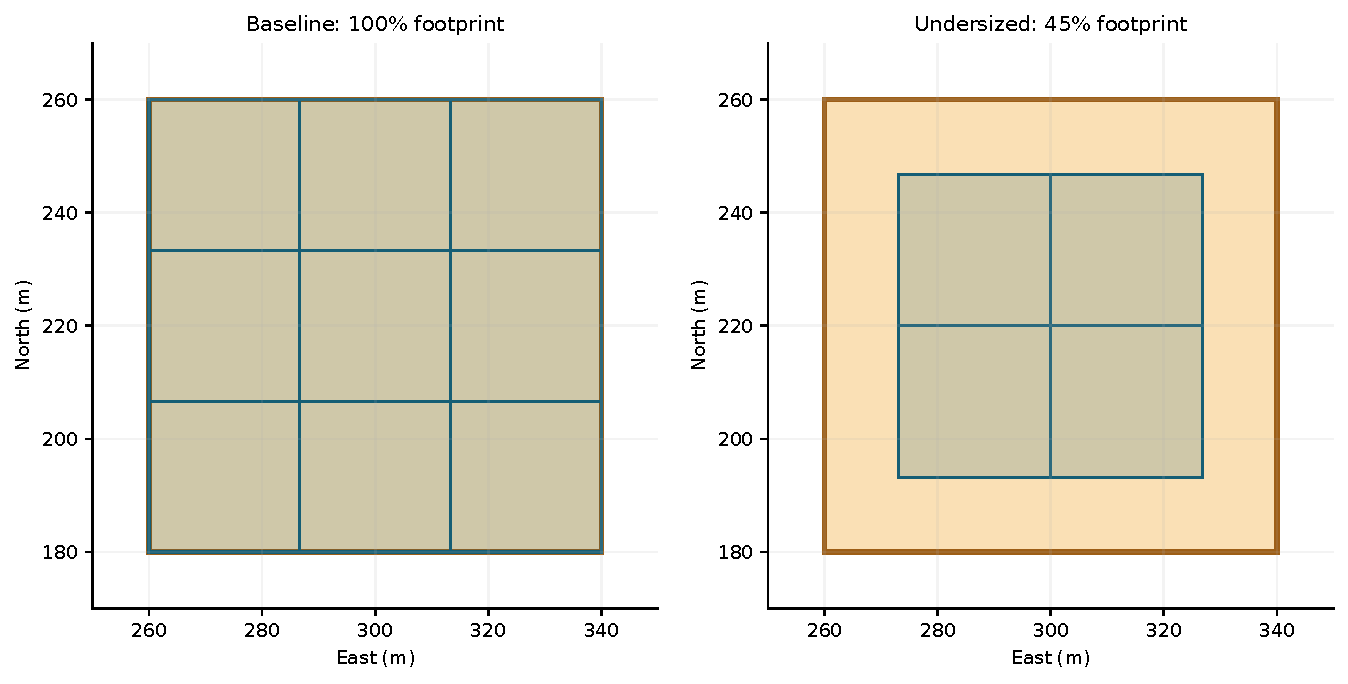
\includegraphics[width=.77\linewidth]{figures/geometry.pdf}
\caption{Corrected deployment geometry using lower-left tile coordinates throughout the column builder, source operator and plotting code. Baseline tiles cover the 6,400~m$^2$ hotspot. The centred undersized design covers 45\% while preserving the hotspot aspect ratio. Bypass and physical damage reduce effective reactive cover separately.}
\label{fig:geometry}\end{figure}
\clearpage
\section{Monitoring, uncertainty and maintenance decisions}
\label{sec:monitoring}

The monitoring component asks what an operator could infer from a limited, delayed and imperfect observation programme. Its most useful conceptual separation is between the hidden simulated state, observation records, and estimates. The observation generator may read the simulated layer history; the estimator receives records and the operator's knowledge of the installed geometry and accepted servicing events. A laboratory acquisition pathway does not make an artificial observation a field measurement: generated records retain the provenance label \texttt{synthetic\_demo}. The implementation reviewed here is an interval-based demonstrator, rather than a calibrated statistical estimator or a validated operational monitoring system.

\subsection{Measurement quantities and data contract}

Each record identifies its station, sample or instrument, mat tile where applicable, measured parameter, analytical fraction, sampling matrix, acquisition method, unit, quality flag and provenance. Sampling time and availability time are separate UTC fields. A result is visible to a decision only when its availability time has arrived; the original sampling time remains attached to the evidence. Integrated deployments also carry start and end times, and a benthic-chamber flux requires a positive enclosed area. Depth carries an explicit reference datum. These distinctions avoid interpreting a concentration above the mat as a sediment concentration beneath it, or an assay of removed media as the loading of freshly installed media.

The unit system separates aqueous concentration (kg\,m$^{-3}$), solid loading (kg\,kg$^{-1}$), accumulated mass (kg), areal flux (kg\,m$^{-2}$\,s$^{-1}$), length (m) and velocity (m\,s$^{-1}$). In particular, ng\,g$^{-1}$ is not interchangeable with ng\,L$^{-1}$, and a chamber flux cannot be recovered from a bottom-water concentration without an additional transport model. Chamber methods can measure sediment--water exchange, but their experimental conditions and applicability require separate validation; the USGS chamber study cited here is methodological precedent in shallow freshwater, not validation of this marine deployment.\cite{benthicFluxMonitoring}

\begin{table}[htbp]
\centering\small
\caption{Intended evidence channels and their physical interpretation. The coupled estimator applies the observation operator and selects compatible matrix/fraction channels before reconstruction.}
\label{tab:monitoring-channels}
\begin{tabular}{p{0.24\linewidth}p{0.34\linewidth}p{0.32\linewidth}}
\toprule
Channel & Quantity represented & Interpretation limit \\
\midrule
Sediment-face porewater & Boundary concentration driving the layer & Pb filtered-dissolved and Hg dissolved-inorganic fractions are distinct from labile water-column channels. \\
Bottom-water chemistry & Concentration above the mat & Does not directly establish residual areal flux or sorbent loading. \\
Benthic chamber & Residual flux over a deployment window & Reduced flux may reflect burial or source change as well as sorption. \\
DGT sampler & Accumulated mass over an exposure & Retained as evidence; no calibrated sampler operator converts it to a point concentration. \\
Media assay & Mass loading of an identified batch & Removed batches cannot constrain the loading of their replacements. \\
Survey and inspection & Coverage, position, burial and damage class & Constrain physical condition; do not measure chemical capacity. \\
Pressure and context & Head loss, currents and water conditions & Support interpretation and instrument health; do not infer Pb or Hg concentration. \\
\bottomrule
\end{tabular}
\end{table}

The observation operator distinguishes assimilable observations, evidence retained without assimilation, and rejected interpretations. The coupled estimator now admits only records classified as assimilable, time-gates them again and requires an installed tile identifier. It keeps DGT-labile, methylmercury and other incompatible operational fractions separate. For source reconstruction, Pb porewater must be filtered dissolved and Hg porewater dissolved inorganic; chamber fractions are total recoverable for Pb and dissolved inorganic for Hg. A methylmercury record therefore cannot replace inorganic-Hg source chemistry. Its optional total-recoverable to model-fraction ratio is disabled by default and, when enabled, creates an uncertain interval. This is a classification capability: the repository does not thereby demonstrate a fitted likelihood or posterior distribution. Copper is present in the physical model, but the default observation generator produces a Pb probe and Pb/Hg laboratory chemistry, and the shared metal-observation set still contains only Pb and Hg. Consequently, three-element simulation should not be described as three-element monitored control.

\subsection{Synthetic sampling and quality control}

Table~\ref{tab:monitoring-defaults} records the nominal monitoring configuration. All detection limits, noise levels, sampling frequencies and delays are demonstration assumptions rather than verified instrument specifications. The laboratory path adds 2\% sample loss, while the probe uses 3\% random missingness. A missing result has no value or censoring bounds. A result below detection or quantification retains a finite interval and is not replaced by zero. Above-range observations carry a lower bound in the data contract.

\begin{table}[htbp]
\centering\small
\caption{Synthetic observation defaults. Campaigns retain a global run clock across decision windows; availability delays remain separate from sampling cadence.}
\label{tab:monitoring-defaults}
\begin{tabular}{p{0.31\linewidth}p{0.21\linewidth}p{0.38\linewidth}}
\toprule
Channel & Nominal period; delay & Noise and analytical bounds \\
\midrule
Environmental station & 1 h; immediate & 2\% relative noise; omitted from coupled maintenance runs. \\
Pb bottom-water probe & 6 h; immediate & 20\% relative noise; LOD 12, LOQ 40 and range ceiling 5,000 ng\,L$^{-1}$. \\
Porewater laboratory & 90 d; 21 d & 8\% relative noise; LOD 1.5 and LOQ 5 ng\,L$^{-1}$. \\
Benthic chamber & 180 d; laboratory delay & 35\% relative noise; LOD 0.05 and LOQ 0.20 $\mu$g\,m$^{-2}$\,d$^{-1}$; 0.196 m$^2$ chamber, 24 h deployment. \\
DGT & 180 d; laboratory delay & 3 d exposure; 15\% relative noise; uptake rate $2.8\times10^{-10}$ m$^3$\,s$^{-1}$; capacity 50,000 ng. \\
Condition survey & 180 d; 1 d & 10\% adjacent-class misclassification; 4\% aborted survey legs. \\
Differential head & Daily; immediate & 8\% relative noise. \\
\bottomrule
\end{tabular}
\end{table}

The generator uses a single deployment origin. Windowed generation evaluates the global schedule and emits completed samples or exposures in the requested interval; splitting a run into monthly decisions does not create additional 90- or 180-day campaigns. Random draws are keyed by the run seed, channel, asset, sample time and element, so a changed window partition or another channel's dropout does not reassign unrelated noise. Record identifiers are stable. Chamber and DGT exposures can cross a decision boundary, while the availability gate still withholds their results until completion and reporting delay.

Additional survey noise assumptions are 0.03 absolute coverage fraction, 0.010 m burial or scour depth, 0.25 m displacement, and $0.8^\circ$ tilt. The damage vocabulary is ordinal: intact, abraded, punctured, torn and lost imply integrity intervals $[0.98,1]$, $[0.85,0.99]$, $[0.50,0.90]$, $[0.10,0.60]$ and $[0,0.10]$, respectively. These overlapping intervals are conventions for visual interpretation, not measured probabilities. Other synthetic chemical conventions include a labile-to-dissolved factor of 1, a total-recoverable-to-labile factor of 1.6, and a methylmercury channel nominally equal to 4\% of porewater Hg. That last channel is not a mechanistic methylation model.

The coupled runner screens only records available at the decision time using a quality-control module that adopts QARTOD-inspired flag names: passed (1), not evaluated (2), suspect (3), failed (4) and missing (9). It is not QARTOD certification.\cite{qartod} Checks comprise gross range, a two-neighbour spike test, repeated values and categorical vocabulary, followed by asset-age summaries. Spike limits take the greater of an absolute floor and a fraction of the neighbour mean. Physical step changes such as displacement and damage are deliberately exempt from spike thresholds. Five consecutive equal values within the configured tolerance trigger the repeated-value check for channels where it is applicable. Non-sensor condition surveys, including repeated physical zeros, are exempt from this flatline rule; stability is not itself survey failure. Channel identity includes matrix, analytical fraction and tile, so unrelated series are not pooled into a spike or repeat test. Flags preserve upstream concerns and do not silently repair or delete data.

Censoring support in the record and interval estimator must be distinguished from acceptance by this coupled QC gate. The current QC skips the scalar range test for a censored result and cannot perform a scalar spike test without values. If no check applies, it assigns not evaluated (2), even when the input flag was passed (1). The estimator accepts only passed post-QC records. Generated non-detects and above-range results therefore retain their bounds in the evidence archive but do not automatically enter the coupled reconstruction. No validated QC rule for censoring intervals is implemented. In scenario A, the available Hg chamber results at days 1 and 181 are respectively below LOD, $[0,0.05]$, and below LOQ, $[0.05,0.20]$ $\mu$g\,m$^{-2}$\,d$^{-1}$; both become not evaluated. The quantified day-361 result becomes available on day 382, beyond the one-year horizon. The final estimate consequently has no usable Hg chamber age and an Hg attenuation interval $[0,1]$. Its twelve sampling recommendations reflect this evidence limitation as well as the policy's channel requirements.

Range checks are specific to both quantity and matrix. For example, the Pb upper bound is 5,000 ng\,L$^{-1}$ in bottom water and 5,000 $\mu$g\,L$^{-1}$ in porewater; Hg bounds are 500 ng\,L$^{-1}$ and 50 $\mu$g\,L$^{-1}$, respectively. Flux bounds are 200,000 $\mu$g\,m$^{-2}$\,d$^{-1}$ for Pb and 2,000 for Hg. These are instrument-plausibility assumptions, not environmental criteria. Default age limits are six hours for ordinary channels, 250 days for porewater and 400 days for flux and surveys. Asset summaries aggregate records by instrument, tile or station; the current summary regards any non-missing record as a latest usable contact, including a failed record. It therefore complements, rather than replaces, explicit channel-level validity checks.

\subsection{Interval reconstruction of flux, loading and remaining capacity}

For a quantified chemical record, the implemented estimator uses
\begin{equation}
I_C=[\max(0,C-2\sigma),\ C+2\sigma].
\end{equation}
For records admitted to the interval estimator, non-detects retain their supplied bounds and above-range records remain $[C_{\min},+\infty)$ rather than acquiring an invented finite upper limit. This standalone interval capability does not override the coupled QC limitation described above: only compatible records with a passed post-QC flag enter the reconstruction. If a quantified chemical record omits its uncertainty, the estimator assumes a relative standard deviation of 0.50 and records that convention, giving $[0,2C]$ for a non-negative value. This fallback is not a measured error model. Numeric physical anomalies require a reported uncertainty before the two-standard-deviation resolution rule can be applied; categorical damage uses the stated class bands.

The estimated source interval is the product of the latest porewater interval and an assumed seepage band,
\begin{equation}
I_{J_s}=I_{C_s}\,[0.4v_0,2.5v_0],
\label{eq:estimated-source}
\end{equation}
where $v_0$ is the initial design seepage velocity. This approximation does not reconstruct the complete diffusive and advective source exchange used by the physical simulator, and it does not assimilate measured seepage. A source increase after installation can therefore remain confounded with performance loss. Without usable porewater chemistry the implementation stores a zero source interval and marks insufficient data; this is an internal unknown-data convention, not evidence of a zero source.

The latest usable chamber interval gives $I_{J_r}$. Without a chamber, residual flux spans zero to the source upper bound. With positive source bounds, attenuation is reconstructed by endpoint arithmetic:
\begin{equation}
I_A=\left[\mathcal{C}\!\left(1-\frac{J_r^+}{J_s^-}\right),\,
\mathcal{C}\!\left(1-\frac{J_r^-}{J_s^+}\right)\right],\qquad
\mathcal{C}(x)=\min\{1,\max\{0,x\}\}.
\end{equation}
If the denominator interval includes zero, attenuation becomes $[0,1]$. Clipping each endpoint maps an entirely negative interval to $[0,0]$, rather than taking a set intersection. It prevents estimated attenuation from representing negative net-release attenuation, although the simulated-truth plots retain that possibility. Captured flux is bounded by
\begin{equation}
I_{J_c}=\big[\max(J_s^- -J_r^+,0),\ \max(J_s^+-J_r^-,0)\big].
\end{equation}
Loading is integrated over the observed history using a zero-order hold between measurements. The first measurement is also held backwards to installation. That back-extrapolation, gaps between campaigns, and unmeasured spatial heterogeneity are substantive assumptions. After replacement, integration starts at the latest accepted installation event. Chamber and condition observations at or before replacement describe the outgoing media and are excluded from current-media reconstruction; an integrated chamber sample must also have started at or after installation. Sediment porewater measurements remain available because source conditions do not reset with the media.

Where a tile lacks its own chemistry, the estimator borrows the mat-wide record pool and widens its interval. For a positive interval $[a,b]$, geometric widening uses
\begin{equation}
g=\sqrt{ab},\qquad
I'=\left[g(b/a)^{-(1+w)/2},\ g(b/a)^{(1+w)/2}\right].
\end{equation}
The widening parameter is 0.35 per year of record age, with an additional 0.5 for borrowed chemistry. These are assumed penalties, not measured variability. For intervals touching zero, arithmetic widening is used instead. An unbounded interval retains its infinite upper endpoint, with lower bound divided by $1+w$. Exported JSON represents non-finite endpoints as null with explicit path metadata; null is not a zero or a finite analytical bound.

The operator capacity interval is $I_Q=L_s f_e I_{q_{\max,e}}$, where $L_s$ is sorbent loading per area and $f_e$ the allocation to element $e$. A configured commissioning interval supersedes the broader material range. The default commissioning intervals are hypothetical commissioning knowledge, not results of an experiment in this repository. The integrated retained-loading interval is clipped to the configured capacity upper bound. This finite-stock constraint is a material assumption, not an upper bound supplied by an above-range measurement. Remaining capacity is
\begin{equation}
I_R=[\max(Q^- -L^+,0),\ \max(Q^+ -L^-,0)],
\end{equation}
and the remaining-time interval is $[R^-/J_c^+,R^+/J_c^-]$ only when $J_c^->0$. Otherwise no time is forecast. Although snapshots carry \texttt{interval\_level=0.9}, no coverage calibration supports a 90\% confidence interpretation: these are deterministic uncertainty bounds, and the ensemble size is zero. Fouling, effective permeability and model--data compatibility remain unestimated fields.

\subsection{Maintenance rules, accounting and interpretation}

The three policies are a bare-seabed reference with no mat, fixed servicing, and evidence-informed servicing. The fixed policy replaces all tiles after two years since the previous service. Decisions are checked every 30 days, so actual dates follow that decision grid. The evidence policy requires at least three chemical evidence identifiers and recent porewater and chamber results for every supported monitored element, Pb and Hg. Each required channel must be present and no older than 200 days. A recent survey or Pb record cannot refresh an old Hg result. Cu has no default chemical observation channel and is not used to demand an impossible Cu sampling cadence. Recent severe physical failure is evaluated before these chemistry conditions, allowing condition evidence to prompt service without an unrelated laboratory result.

For each element, saturation is bounded by $[L^-/Q^+,L^+/Q^-]$, with the upper endpoint capped at one. The default decision value is the interval midpoint; lower and upper choices are configurable risk postures. Inspection and replacement thresholds are 0.55 and 0.80. An attenuation interval whose upper endpoint falls below 0.70 also prompts inspection. A damage-class integrity upper bound strictly below 0.90 prompts inspection and replacement. With the default class mapping, this automatically catches torn and lost classes, but not punctured at its upper bound of exactly 0.90. These are demonstration triggers, not engineering acceptance criteria.

Cause attribution starts with equal weights for saturation, fouling, displacement and local damage. The latest non-intact damage class, including punctured, adds three weight units to local damage. A coverage upper bound below 0.98, or displacement/uplift/tilt resolved beyond two standard deviations, adds evidence for displacement. A resolved head increase or permeability decrease against the earliest comparable available baseline can support fouling; the presence of a channel alone does not. The latest burial lower bound must be positive after length conversion and two-standard-deviation uncertainty before burial is flagged. An unburied or noise-consistent-zero survey consequently does not imply a buried mat.

Only elements with compatible measured porewater and chamber records and a computable attenuation ratio enter performance-loss attribution. An unmonitored Cu channel or an unknown source cannot itself create evidence of saturation or source change. Chemistry consistent with reduced attenuation, together with physical evidence, can add one unit to saturation, while missing discriminating physical evidence retains source-change and seepage-change explanations. The normalised weights are explanatory heuristics, not posterior probabilities. Source-side ambiguity or resolved burial blocks replacement attributed to saturation and requests further evidence. The exact policy thresholds remain distinct from the class-to-integrity mapping: a punctured class can support a damage explanation without automatically satisfying the strict integrity-upper-bound replacement trigger.

Every recommendation is labelled simulation-only and requires human confirmation in its exported contract. The demonstrator automatically accepts replacement recommendations to simulate an operator following the policy. Sampling and inspection recommendations do not modify the future observation programme; additional sampling cost is therefore not an executed adaptive campaign in these runs. Replacement resets the selected tiles and transfers their retained contaminant to the retrieved-media ledger. Removed media are treated as waste with a handling cost, never as a saleable metal product.

Assumed prices are EUR 240\,m$^{-2}$ material, EUR 6,500 per vessel visit/day, EUR 1,900 tile replacement handling and EUR 12\,kg$^{-1}$ used-media handling. Additional configured prices are EUR 4,200 per ROV survey, EUR 2,800 per chamber deployment, EUR 180 per porewater sample, EUR 210 per Hg laboratory sample, EUR 260 per DGT deployment and EUR 350 per sensor check. The recorded servicing total includes accepted replacements; it does not include every possible monitoring, permitting or initial-installation cost. Hence cost per retained kilogram is not a complete life-cycle or exposure-reduction cost.

\subsection{Limits of the demonstrated control loop}
\label{sec:control-limitations}

The revised run uses availability gating, QC and analytical-fraction classification before estimation. Raw observations, estimate histories, recommendation evidence identifiers and accepted service events are exported to support reconstruction of the evidence available at each decision. The exported final QC report is a retrospective screen; replay must apply the original availability gate before QC. Recommendations that request data or follow a fixed schedule can have empty evidence-identifier lists. Campaign cadence and scenario-E dropout/drift follow elapsed time since deployment: the configured dropout is from 1.0 to 1.25 years, drift begins at 1.25 years and laboratory latency is 75 days. These are simulated disruptions, not observed instrument behaviour or evidence of a commercially available monitoring system.

Several modelling limits remain. Porewater and an assumed seepage band reconstruct only an advective source estimate, while the physical reference also includes diffusive exchange. Synthetic chamber values follow local column flux, whereas reported whole-hotspot emission additionally includes uncovered, damaged and bypass contributions. A chamber's spatial representativeness therefore requires explicit assessment. The generator's layer-history adapter has no dynamic hydraulic-head or tilt model; these channels are marked missing rather than manufactured as exact zeros. Separate scripted scenes may provide such values, but do not validate their physical relationship to fouling or displacement.

Station placement also remains fixed. Scenario F contains only four tiles and omits \texttt{tile\_2\_2}, to which the default chamber station is assigned. The runner filters out that station rather than relocating it. Consequently, F generates no Pb or Hg chamber records and records 48 requests for chemical sampling without a service. This is a limitation of the configured monitoring layout and its lack of adaptive sampling, not evidence that the undersized mat remained chemically effective.

Cu is simulated but unmonitored. Without usable source chemistry, the legacy snapshot stores zero source bounds alongside an insufficient-data flag, returns attenuation $[0,1]$ and makes no remaining-time forecast. Those stored zeros denote unavailable information, not a measured absence of source, loading or risk. Missing-data flags must therefore accompany any operational interpretation of the numeric fields. Borrowed chemistry, backward holding of the first sample and assumed material bounds add uncertainty beyond instrument noise.

The estimator is a deterministic interval reconstruction without a calibrated observation likelihood, particle ensemble or demonstrated interval coverage. Recommendation-level \texttt{data\_age\_s} remains null; per-channel ages are available in the estimate snapshots. Fouling, permeability and compatibility fields remain unestimated, and estimated attenuation is clipped to $[0,1]$. The configured maximum relative interval width and partial-replacement switch remain unused by the current policy; trend-count and indistinguishability parameters likewise do not alter the current estimator. Sampling and inspection recommendations do not adapt future campaigns in this demonstrator, and assumed service expenditure omits a complete lifecycle accounting. Consequently, changed recommendations and costs after these repairs establish software behaviour under explicit assumptions, not operational superiority or a validated maintenance optimum.

\section{Regenerated demonstrator results}
\label{sec:results}
\subsection{Scenario design and performance measures}
All reported results are synthetic and were regenerated after the scientific revision. The shared seed is 20260908. A model year is 365.25 days. The baseline uses a 10~mm core with 4~kg\,m$^{-2}$ dry loading, nine tiles and complete geometric coverage of the hypothetical hotspot. Scenario F changes both geometry and transport and is therefore a compound stress case.

\begin{table}[htbp]\centering\small
\caption{Configured six-scenario experiments.}\label{tab:scenarios}
\begin{tabular}{llrp{.48\linewidth}}\toprule
ID & Scenario & Years & Change \\
\midrule
A & Fresh mat & 1 & Baseline source and fresh medium. \\
B & Progressive loading & 6 & Same physical configuration, longer exposure. \\
C & Increased source & 6 & At year 2, porewater concentrations triple and seepage doubles. \\
D & Local damage & 4 & Displacement at year 1.5; another tile loses 35\% integrity at year 2.2. \\
E & Delayed chemistry & 4 & 75-day lab delay, probe dropout at years 1--1.25 and subsequent drift. \\
F & Undersized mat & 4 & 45\% footprint, four tiles, 2~mm core, 10\% edge bypass and tripled seepage. \\
\bottomrule\end{tabular}\end{table}

The principal attenuation is the whole-hotspot quantity
\begin{equation}
A_{\mathrm{area},e}(t)=1-\frac{\int_{\Omega_h}J_{\mathrm{res},e}(x,y,t)\,\mathrm{d}A}{|\Omega_h|J_{\mathrm{bare},e}(t)}.
\end{equation}
It includes uncovered area, physical damage and bypass. The raw-column attenuation remains a separate diagnostic. The barrier-only comparator applies the same area weighting to the exact stationary discrete column with uptake disabled. Its difference from transient total attenuation is a diagnostic increment, not an isolated measurement of chemistry: transient porewater storage also contributes.

The endpoint concentration ratio is $R_{\max,e}=\max c_{\mathrm{with},e}/\max c_{\mathrm{bare},e}$. Its two maxima need not occur in the same cell. Neither source attenuation nor this ratio is a toxicity or compliance metric. Retained column mass comprises porewater and sorbed inventory; the active and retrieved parts are recorded separately.

\subsection{Final states and chemical contribution}
\begin{table}[htbp]\centering\small
\caption{Final whole-hotspot attenuation and nominal sorbed-capacity use (percent). No statistical confidence interval is implied.}\label{tab:all-metals}
\begin{tabular}{lrrrrrr}\toprule
Scenario & $A_{\rm Pb}$ & $A_{\rm Hg}$ & $A_{\rm Cu}$ & $q_{\rm Pb}/q_{\max}$ & $q_{\rm Hg}/q_{\max}$ & $q_{\rm Cu}/q_{\max}$ \\
\midrule
A & 89.93 & 91.92 & 87.13 & 44.69 & 0.36 & 8.70 \\
B & 61.32 & 61.57 & 61.19 & 66.76 & 0.83 & 9.53 \\
C & 57.91 & 58.09 & 57.92 & 100.00 & 2.75 & 30.62 \\
D & 70.21 & 70.99 & 69.99 & 63.31 & 0.74 & 9.11 \\
E & 71.75 & 72.40 & 71.59 & 64.01 & 0.76 & 9.15 \\
F & 25.87 & 25.87 & 25.85 & 66.60 & 0.85 & 9.41 \\
\bottomrule\end{tabular}\end{table}

\begin{table}[htbp]\centering\small
\caption{Final footprint after physical condition, Pb column inventories and monitoring workload. Coverage excludes edge/fouling bypass; records include explicit missing results.}\label{tab:scenario-results}
\begin{tabular}{lrrrrr}\toprule
Scenario & Coverage (\%) & Active Pb (kg) & Retrieved Pb (kg) & Services & Records \\
\midrule
A & 100.00 & 6.884 & 0 & 0 & 4950 \\
B & 100.00 & 10.28 & 0 & 0 & 29349 \\
C & 100.00 & 15.45 & 0 & 0 & 29349 \\
D & 96.11 & 9.752 & 0.9153 & 1 & 19593 \\
E & 100.00 & 9.859 & 0 & 0 & 19593 \\
F & 45.00 & 0.9233 & 0 & 0 & 11995 \\
\bottomrule\end{tabular}\end{table}

Increasing occupancy does not imply full exhaustion. A low accessible concentration or partition slope can hold the equilibrium load below the allocated capacity. Conversely, decreasing effective coverage can worsen hotspot emission even if surviving columns remain effective. The scenario-D time series now resolves the local physical events at their true times. Any accepted service changes active-media inventory and restores the serviced tile's condition; retrieved mass remains in its separate ledger.

\begin{table}[htbp]\centering\small
\caption{Resolved Pb jumps at a shared event time. The flux ratio is immediately after divided by immediately before; attenuation can rise while absolute emission rises because its bare-source denominator also changes.}\label{tab:event-jumps}
\begin{tabular}{llrrrr}\toprule
ID & Event & Age (yr) & Before (\%) & After (\%) & Flux ratio \\
\midrule
C & Source increase & 2 & 82.72 & 85.08 & 2.737 \\
D & Displacement & 1.5 & 85.99 & 76.44 & 1.682 \\
D & Replacement & 2.053 & 73.24 & 84.13 & 0.593 \\
D & Integrity loss & 2.2 & 83.27 & 80.10 & 1.189 \\
\bottomrule\end{tabular}\end{table}

In scenario C, the source step raises the absolute residual flux even though the instantaneous attenuation ratio improves. Subsequent storage adjustment and Pb capacity locking explain the later bend. In D, the upward jump follows the recorded replacement of a displaced tile; it is followed by a separate integrity-loss event on another tile. These events are explicit changes in the model state, not measurement noise.

\figpage{attenuation_all}{Whole-hotspot attenuation in all six regenerated scenarios. The shared axis includes the complete response of the undersized design. Event-time discontinuities are retained rather than smoothed.}{fig:attenuation}
\figpage{saturation_all}{Sorbed inventory as a fraction of allocated nominal capacity. The profiles are deterministic simulations; low capacity use can coexist with little incremental uptake.}{fig:saturation}
\figpage{condition_all}{Mean fouling, physical integrity and actual hotspot coverage through time. Matching physical histories overlap. Coverage and bypass are distinct: a nominally intact footprint can still lose effective performance as fouling diverts flow.}{fig:condition}
\begin{table}[htbp]\centering\small
\caption{Six-year baseline decomposition using a common discrete transport operator and hotspot weighting. Differences are percentage points.}\label{tab:barrier}
\begin{tabular}{lrrr}\toprule
Element & Total (\%) & Barrier reference (\%) & Difference (pp) \\
\midrule
Pb & 61.32 & 61.19 & 0.1279 \\
Hg & 61.57 & 61.19 & 0.3759 \\
Cu & 61.19 & 61.19 & 0.005172 \\
\bottomrule\end{tabular}\end{table}

The baseline chemical increment is much smaller than the total attenuation. Cumulative storage and an endpoint increment answer different questions: mass retained during an earlier uptake transient can remain in the core even when the later flux approaches a resistance-controlled regime. Subtracting an approximate continuum barrier from a discrete transient result previously introduced small misleading differences, especially for Cu; the revised reference removes that operator mismatch.

\subsection{Spatial source and water transport}
All standard plume windows last 24 hours. The comparison below uses a three-year mat state when that age is within the scenario horizon, and the actual one-year endpoint for A. The source is held fixed during each window and the water starts clean. The final-age source plate in Appendix~\ref{app:spatial} additionally shows each scenario endpoint.
\begin{table}[htbp]\centering\small
\caption{Pb comparison at the stated mat age. Source is kg per 24-hour window; endpoint concentration maxima are ng/L.}\label{tab:spatial-results}
\begin{tabular}{lrrrrrrr}\toprule
ID & Age (yr) & Bare kg & Mat kg & Reduction (\%) & Bare peak & Mat peak & $R_{\max}$ \\
\midrule
A & 1 & 0.2931 & 0.0295 & 89.93 & 59.99 & 6.039 & 0.1007 \\
B & 3 & 0.2931 & 0.06726 & 77.05 & 39.37 & 9.035 & 0.2295 \\
C & 3 & 0.929 & 0.2535 & 72.71 & 124.8 & 34.06 & 0.2729 \\
D & 3 & 0.2931 & 0.07169 & 75.54 & 39.37 & 10.32 & 0.2621 \\
E & 3 & 0.2931 & 0.06726 & 77.05 & 39.37 & 9.035 & 0.2295 \\
F & 3 & 0.3262 & 0.2351 & 27.95 & 43.83 & 28.29 & 0.6454 \\
\bottomrule\end{tabular}\end{table}

Unlike the previous geometry, the configured damaged tiles intersect the hotspot. Their source changes are therefore represented spatially. Scenario E changes observation timing rather than material coefficients; equality with a matched physical trajectory is expected whenever the policy produces the same servicing history. Scenario F leaves 55\% of the hotspot geometrically uncovered before bypass, so its column performance cannot be presented as whole-area performance.

\figpage{flux_30}{Regenerated residual Pb source maps at three years, or the actual one-year endpoint for A, with one shared source scale. Ages are shown in each panel.}{fig:fluxlate}
\figpage{spatial_B}{Baseline B at three years: matched with/without endpoint water concentrations, their cellwise ratio, and effective reactive cover.}{fig:spatialB}
\figpage{profiles_all}{Final Pb profiles through the core for every scenario. Colours show local sorbed load in mg per kg of core; panel scales are stated separately. Similar tiles are deterministic columns, not independent experimental replicates.}{fig:profiles}
\begin{figure}[htbp]\centering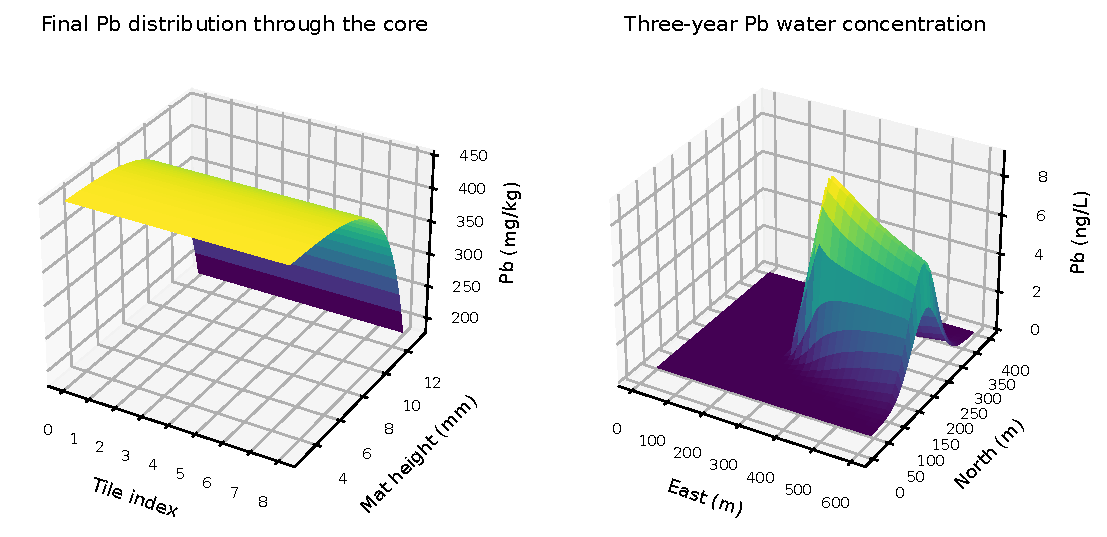
\includegraphics[width=\linewidth]{figures/surfaces.pdf}
\caption{Final six-year baseline Pb load through the core and the three-year endpoint plume shown as surfaces. Height denotes different labelled quantities; concentration is not seabed elevation.}\label{fig:surfaces}\end{figure}

\subsection{Three maintenance policies on a common emission basis}
The comparison uses identical source and forcing assumptions, seed and nominal monitoring configuration. Calendar and evidence-informed servicing share the actual sample calendar; the bare reference has no installed-mat observations. All policies integrate the same whole-hotspot residual source, including uncovered and bypassed area. Calendar service is triggered on the next decision boundary after its interval is reached; the baseline services occur on days 750 and 1500. Evidence-informed service depends on arrived compatible measurements, their quality, attribution and uncertainty. The economic column below is the assumed service ledger; it excludes full lifecycle costs.
\begin{table}[htbp]\centering\small
\caption{Six-year cumulative whole-hotspot emission (kg), service events and assumed service expenditure.}\label{tab:policies}
\begin{tabular}{lrrrrr}\toprule
Policy & Pb emitted & Hg emitted & Cu emitted & Services & Cost (EUR) \\
\midrule
No mat & 642.3 & 5.138 & 1285 & 0 & 0 \\
Calendar & 62.74 & 0.4271 & 163.8 & 2 & 3.734e+06 \\
Evidence & 141.6 & 1.08 & 297.9 & 0 & 0 \\
\bottomrule\end{tabular}\end{table}

\begin{table}[htbp]\centering\small
\caption{Pb inventory accounting in the policy comparison. Column inputs and outputs use the full tile-column control volume and are not added to the area-mixed emission above.}\label{tab:policy-ledger}
\begin{tabular}{lrrrr}\toprule
Policy & Column input (kg) & Active (kg) & Retrieved (kg) & Column out (kg) \\
\midrule
No mat & 0 & 0 & 0 & 0 \\
Calendar & 42.77 & 8.832 & 18 & 15.94 \\
Evidence & 38.71 & 10.28 & 0 & 28.43 \\
\bottomrule\end{tabular}\end{table}

\figpage{policy}{Policy comparison using whole-hotspot Pb emission for every policy. Active plus retrieved column inventory is shown separately. Costs are assumed service expenditure, not total project cost or profit.}{fig:policy}
Sparse Pb/Hg chemistry constrains evidence-informed decisions. Cu is simulated but not observed, and missing Cu no longer contributes evidence of performance loss. Unknown source and flux intervals are identified explicitly; no interval midpoint is a field measurement. Recommendations to sample or inspect do not adapt the future campaign schedule in this demonstrator. This comparison therefore does not establish the value of an optimised monitoring programme.

\subsection{Integration and conservation checks}
The regenerated audit compares final timeline flux with the integrated spatial source for every element and policy, validates every plume age against its simulation horizon, checks observation-ID uniqueness, and checks all individual column and water ledgers. Initial samples are unadvanced; the integration ends at the exact requested time, including a partial last step. The zero-sorption reference is tested against independent stationary face balances and grid refinement, and nonlinear transient profiles against an adaptive ODE reference.
\begin{table}[htbp]\centering\small
\caption{Audit of regenerated scenario outputs. Relative errors are dimensionless. Conservation and agreement are numerical checks, not material validation.}\label{tab:scenario-audit}
\begin{tabular}{lrrll}\toprule
ID & Worst budget error & Source agreement error & Valid ages & Unique IDs \\
\midrule
A & 3.371e-14 & 9.245e-15 & True & True \\
B & 1.661e-13 & 2.062e-15 & True & True \\
C & 1.439e-13 & 1.872e-15 & True & True \\
D & 9.371e-14 & 2.496e-15 & True & True \\
E & 1.101e-13 & 2.637e-15 & True & True \\
F & 5.685e-14 & 3.026e-16 & True & True \\
\bottomrule\end{tabular}\end{table}

% Generated by tools/render_numerical_results.py; values come from audit JSON.
\subsection{Independent numerical verification and discontinuities}
\label{sec:numerical_revision}

The revised code was checked against independently assembled stationary
face balances, a continuum transport solution and adaptive backward
differentiation formula (BDF) integration of the coupled semi-discrete
transport--sorption equations. These checks address equation solving and
discretisation separately from a mass ledger. The complete integrated test
suite is reported separately; the focused checks below address independent
oracles, source discontinuities and exact reuse of equivalent tile states.

For a short nonlinear test, the reference column was set to eight cells and
capacity $10^{-5}$~kg/kg, so that breakthrough occurs within fourteen days.
This is an accelerated verification problem, not a revised material
calibration. Concentration and sorbed-profile errors were normalised by
$10^{-3}$~kg/m$^3$ and capacity, respectively, and compared at daily marks.
The reference uses SciPy~1.18.1's variable-order BDF integration with relative
tolerance $2\times10^{-9}$ and absolute tolerance $10^{-14}$.\citep{scipy_solve_ivp}
Table~\ref{tab:independent-temporal} reports the maximum normalised
profile error, not a fitted coefficient or an assumed precision.


\begin{table}[htbp]\centering\small
\caption{Convergence of the nonlinear column to independent adaptive BDF integration in the accelerated verification problem.}\label{tab:independent-temporal}
\begin{tabular}{rr}\toprule
Step (h) & Maximum normalised profile error \\\midrule
6 & 0.0947294 \\
3 & 0.0534873 \\
1.5 & 0.03128 \\
\bottomrule\end{tabular}\end{table}


\begin{table}[htbp]\centering\small
\caption{Spatial refinement of the non-sorbing reference column against its continuum solution. The approximately halving error is consistent with first-order upwind transport.}\label{tab:independent-spatial}
\begin{tabular}{rr}\toprule
Layer cells & Relative stationary flux error (\%) \\\midrule
20 & 1.12686 \\
40 & 0.564771 \\
80 & 0.2825 \\
160 & 0.141248 \\
\bottomrule\end{tabular}\end{table}


The largest per-step mass residual in this nonlinear verification was $1.60308\times10^{-20}$~kg/m$^2$, with zero recorded clipping. The finite temporal errors in Table~\ref{tab:independent-temporal} show why conservation cannot establish accuracy. The runtime now refuses unconverged sorption branch masks with an instruction to reduce the step or increase the iteration limit.


Within-call reuse of exactly equivalent vertical tile states was also checked against independent per-tile advancement. Fourteen additional regression cases preserve complete step results, identities and independent arrays. A 30-day full-history comparison was bitwise identical across all result fields. One exploratory timing gave 2.14-fold speedup; the recorded repeat under concurrent workload gave 1.17-fold (6.62 versus 7.75~s). Runtime depends on workload; nine equivalent solver calls being reduced to one does not imply ninefold end-to-end acceleration. The benchmark artifact and reproduction script accompany the repository.


The exact discrete barrier also removes a mismatch in the former diagnostic:
the old continuum approximation double-counted a top half-cell resistance and
approximated advective bottom resistance. At the default clean state, the
corrected barrier flux is 2.1346\% higher for Pb and Hg and 2.7534\% higher for
Cu than that old comparison. This changes the interpretation of the plotted
barrier; it does not alter the transport trajectory or calibrate the material.

Two remaining types of abrupt behaviour have explicit causes. First, a step
in the prescribed source changes the denominator of
$1-J_{\mathrm{out}}/J_{\mathrm{bare}}$ immediately, whereas porewater storage
is continuous. A tenfold source decrease produces a tenfold instantaneous
increase in that residual ratio, followed by washout
(Figure~\ref{fig:reactive-numerical-audit}D). Such a ratio dip is compatible
with a conserving solver. Second, the capacity-lock law itself is
discontinuous: an exactly full cell is held, but a cell just below capacity
can desorb. In a six-hour, one-cell clean-water flush, an exactly full state
gives zero outgoing flux; starting at $q/Q=1-10^{-10}$ gives
$9.8426\times10^{-12}$~kg/m$^2$/s. This is an unvalidated constitutive
assumption retained explicitly, not evidence that real keratin exhibits that
switch. No plotted trajectory was smoothed to conceal these effects.


\begin{figure}[htbp]\centering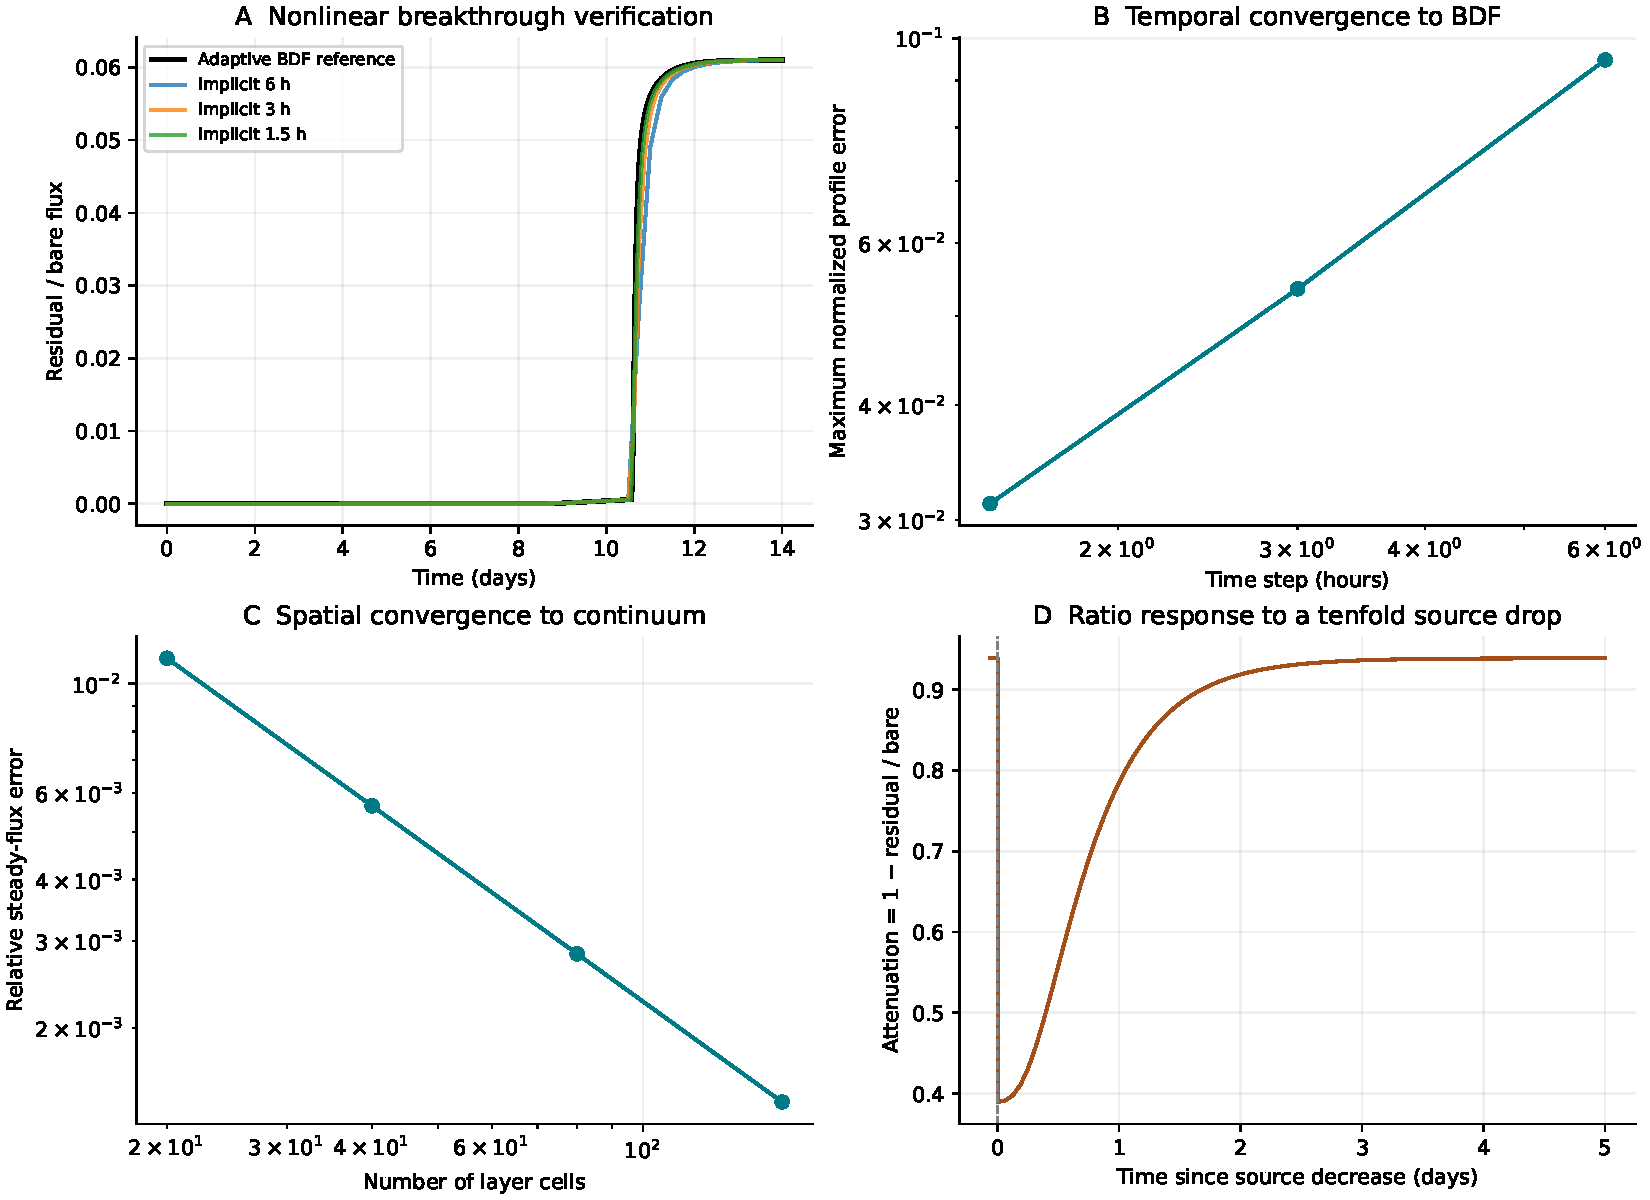
\includegraphics[width=\linewidth]{figures/reactive_numerical_audit.pdf}
\caption{Independent column verification and a forcing-induced ratio dip. A: nonlinear breakthrough against adaptive BDF; B: the maximum normalised profile error under time refinement; C: stationary flux error under spatial refinement; D: instantaneous ratio change and subsequent washout after a tenfold source decrease. The low-capacity test in A--B accelerates verification and is not a scenario material adjustment.}\label{fig:reactive-numerical-audit}\end{figure}


\subsection{Regenerated time-step, horizon and decision studies}
\label{sec:timescale_revision}

The following values were regenerated after the scientific corrections.
Attenuation refers to the whole-hotspot, area-mixed source, including bypass,
and each age is an actually simulated endpoint. The source hash, scenario
identifier and full-precision arrays accompany the manuscript in
\path{data/timescale_audit.json}; the executable study is
\path{tools/timescale_check.py} in the repository.


\begin{table}[htbp]\centering\small
\caption{Regenerated two-year temporal refinement. Source attenuation and the whole-hotspot water input have a different control volume from active column inventory.}\label{tab:revised-refinement}
\resizebox{\linewidth}{!}{\begin{tabular}{rrrrrr}\toprule
Step (h) & Pb attenuation & Pb occupancy & Active Pb (kg) & Pb into water (kg) & Relative imbalance \\\midrule
24 & 0.82725239 & 0.580811 & 8.94603 & 20.884 & $6.64\times10^{-14}$ \\
12 & 0.82723547 & 0.580935 & 8.94794 & 20.8902 & $7.95\times10^{-14}$ \\
6 & 0.8272271 & 0.580997 & 8.9489 & 20.8932 & $2.01\times10^{-14}$ \\
3 & 0.82722292 & 0.581028 & 8.94938 & 20.8948 & $1.95\times10^{-13}$ \\
1 & 0.82722013 & 0.581048 & 8.94969 & 20.8958 & $1.25\times10^{-13}$ \\
\bottomrule\end{tabular}}\end{table}


The terminal attenuation spread is $3.226\times10^{-5}$, and the default six-hour result differs from the finest tested step by $6.976\times10^{-6}$. These are measured sensitivities of these endpoint quantities, not error bounds for every transient feature or for the coastal field.


\begin{table}[htbp]\centering\small
\caption{Exact-age samples from one continuous trajectory through the longest horizon. Barrier attenuation uses the same instantaneous geometry, fouling and bypass as the transient source.}\label{tab:revised-horizon}
\resizebox{\linewidth}{!}{\begin{tabular}{rrrrrrrr}\toprule
Age (yr) & Pb attenuation & Hg attenuation & Cu attenuation & Pb barrier & Hg barrier & Cu barrier & Services \\\midrule
1 & 0.899333 & 0.919219 & 0.871295 & 0.871545 & 0.871545 & 0.871257 & 0 \\
2 & 0.827227 & 0.846831 & 0.819577 & 0.819748 & 0.819748 & 0.819536 & 0 \\
4 & 0.717464 & 0.724005 & 0.715906 & 0.715946 & 0.715946 & 0.715858 & 0 \\
8 & 0.594422 & 0.595379 & 0.594313 & 0.594324 & 0.594324 & 0.594313 & 0 \\
16 & 0.594324 & 0.594327 & 0.594313 & 0.594324 & 0.594324 & 0.594313 & 0 \\
\bottomrule\end{tabular}}\end{table}


Horizon dependence describes evolving storage and condition. The difference
between transient and stationary-barrier attenuation includes history and
dissolved storage; it is not a separately validated sorbent efficiency or a
service-life measurement.


\begin{table}[htbp]\centering\small
\caption{Coastal duration and tidal-phase sensitivity. Every run starts from clean water with the same exact one-year mat state; the source is fixed during the window. Integer-cycle endpoints provide an additional comparison at matching phases.}\label{tab:revised-window}
\resizebox{\linewidth}{!}{\begin{tabular}{rrrrrr}\toprule
Window (h) & Tidal cycles & Pb peak: mat (ng/L) & Pb peak: bare (ng/L) & Peak ratio & Source ratio \\\midrule
3 & 0.2415 & 17.6971 & 175.798 & 0.1006671 & 0.1006671 \\
6 & 0.4831 & 3.78804 & 37.6294 & 0.1006671 & 0.1006671 \\
12 & 0.9662 & 5.74824 & 57.1015 & 0.1006671 & 0.1006671 \\
24 & 1.932 & 6.03871 & 59.9869 & 0.1006671 & 0.1006671 \\
24.84 & 2 & 5.82456 & 57.8597 & 0.1006671 & 0.1006671 \\
37.26 & 3 & 5.84223 & 58.0352 & 0.1006671 & 0.1006671 \\
48 & 3.865 & 10.2414 & 101.735 & 0.1006671 & 0.1006671 \\
49.68 & 4 & 5.8281 & 57.8948 & 0.1006671 & 0.1006671 \\
\bottomrule\end{tabular}}\end{table}


The with-mat terminal Pb maximum spans 3.78804--17.6971~ng/L, while the with/bare peak ratio spans 0.10066706--0.10066706. A nearly invariant ratio can coexist with tide-dependent absolute peaks when a linear transport model is driven by proportional source fields.


These endpoint observations are not a monotonic steady-state convergence
sequence. Duration changes both spin-up and tidal phase, whereas matching
integer-cycle endpoints test approach to a periodic response. This finite set
does not prove that a periodic state has settled. A tide-dependent peak is not
by itself a solver defect; the separate discretisation study below measures
time-step and grid sensitivity under a fixed physical window and phase.


\begin{table}[htbp]\centering\small
\caption{Four-year decision-cadence comparison with a global observation calendar. Recommendations count individual returned recommendations, not necessarily distinct campaign dates.}\label{tab:revised-cadence}
\resizebox{\linewidth}{!}{\begin{tabular}{rrrrrr}\toprule
Review period (d) & Recommendations & Services & Observations & Pb attenuation & Assumed cost (EUR) \\\midrule
15 & 97 & 0 & 19593 & 0.717464 & 0 \\
30 & 48 & 0 & 19593 & 0.717464 & 0 \\
90 & 16 & 0 & 19593 & 0.717464 & 0 \\
180 & 8 & 0 & 19593 & 0.717464 & 0 \\
365 & 4 & 0 & 19593 & 0.717464 & 0 \\
\bottomrule\end{tabular}}\end{table}


The station/time/parameter/method calendar hashes are identical across these cadence runs. This check compares observation calendars, not noisy measured values or the subset available at any particular decision. Cadence determines when existing evidence is reviewed; it must not generate additional samples.


\begin{figure}[htbp]\centering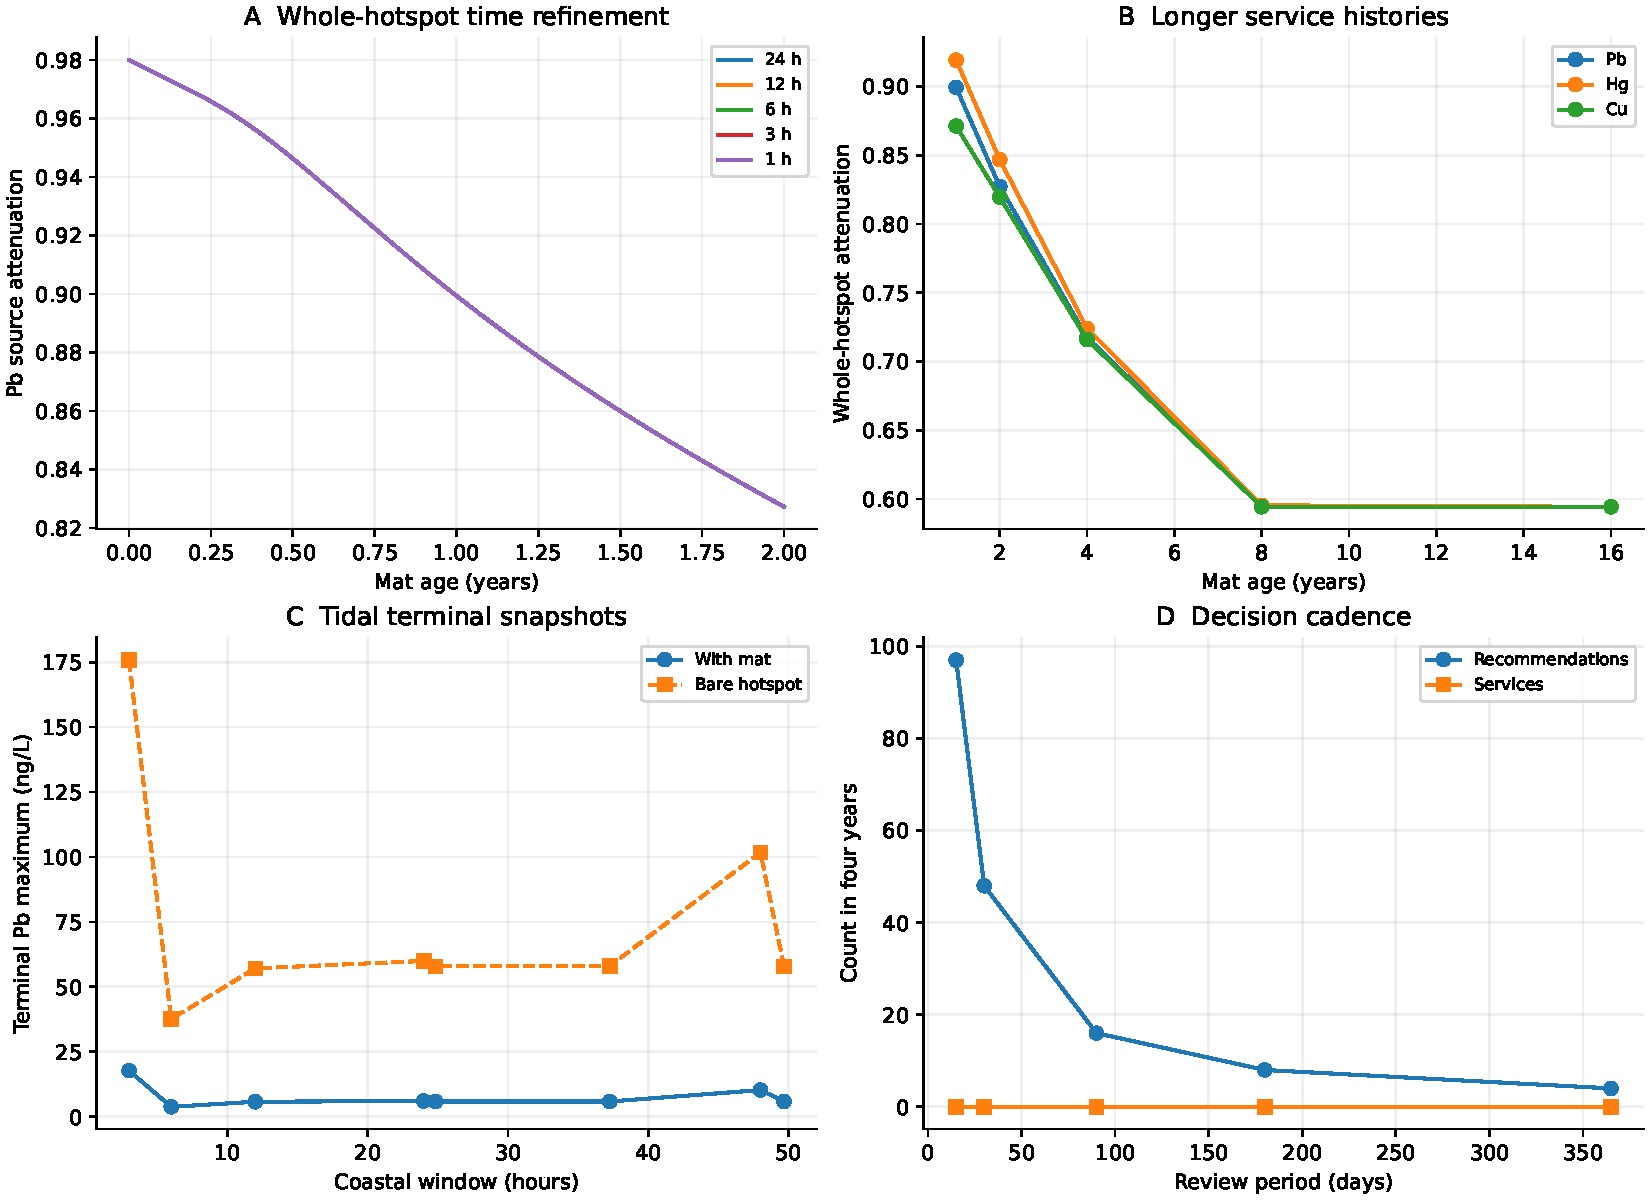
\includegraphics[width=\linewidth]{figures/timescale_audit.pdf}
\caption{Regenerated scenario studies: A, two-year whole-hotspot attenuation under time refinement; B, longer exact-age histories; C, terminal coastal maxima at different window lengths and tidal phases; D, recommendations and accepted services at different review cadences. Lines join computed samples without smoothing; the coarse horizon samples are not continuous observations.}\label{fig:timescale-audit}\end{figure}


\subsection{Coastal discretisation sensitivity}
\label{sec:coastal_refinement}

The coastal audit holds the $600\times400$~m physical domain, one-year mat
state, initial concentration, forcing phase, fixed source and 24-hour window
constant. Time steps of 600, 300 and 150~s use a 10-m grid; grids of 20, 10
and 5~m use a 150-s step. The hotspot and straight land edges align with all
three grids, avoiding a change in prescribed footprint area. The same FiPy
transport implementation is used.\citep{fipy2009}


\begin{table}[htbp]\centering\small
\caption{Fixed-window coastal time-step and grid refinement. These are numerical sensitivities rather than uncertainty intervals from material variability.}\label{tab:coastal-discretisation}
\resizebox{\linewidth}{!}{\begin{tabular}{rrrrrr}\toprule
Grid (m) & Step (s) & Pb peak: mat (ng/L) & Pb peak: bare (ng/L) & Peak ratio & Pb in water (kg) \\\midrule
10 & 600 & 6.03871 & 59.9869 & 0.1006671 & 0.000972618 \\
10 & 300 & 5.90376 & 58.6464 & 0.1006671 & 0.000868248 \\
10 & 150 & 5.86022 & 58.2138 & 0.1006671 & 0.00082418 \\
20 & 150 & 5.75969 & 57.2152 & 0.1006671 & 0.000845344 \\
5 & 150 & 5.88378 & 58.4479 & 0.1006671 & 0.000818459 \\
\bottomrule\end{tabular}}\end{table}


The 600-s versus 150-s terminal with-mat Pb peak difference at 10~m is 3.046\%; the 10-m versus 5-m difference at 150~s is -0.400\%. Each signed difference is expressed relative to the finer result. Coexisting temporal and spatial errors prevent these differences from being interpreted as bounds relative to an exact PDE solution. A stable source ratio or closed water ledger does not eliminate peak-concentration discretisation error.


For the remaining Pb inventory in the water, the corresponding differences are 18.010\% under time refinement and 0.699\% under grid refinement. The larger temporal sensitivity of this integrated field quantity further limits claims of coastal numerical accuracy based on a terminal peak alone.


\begin{figure}[htbp]\centering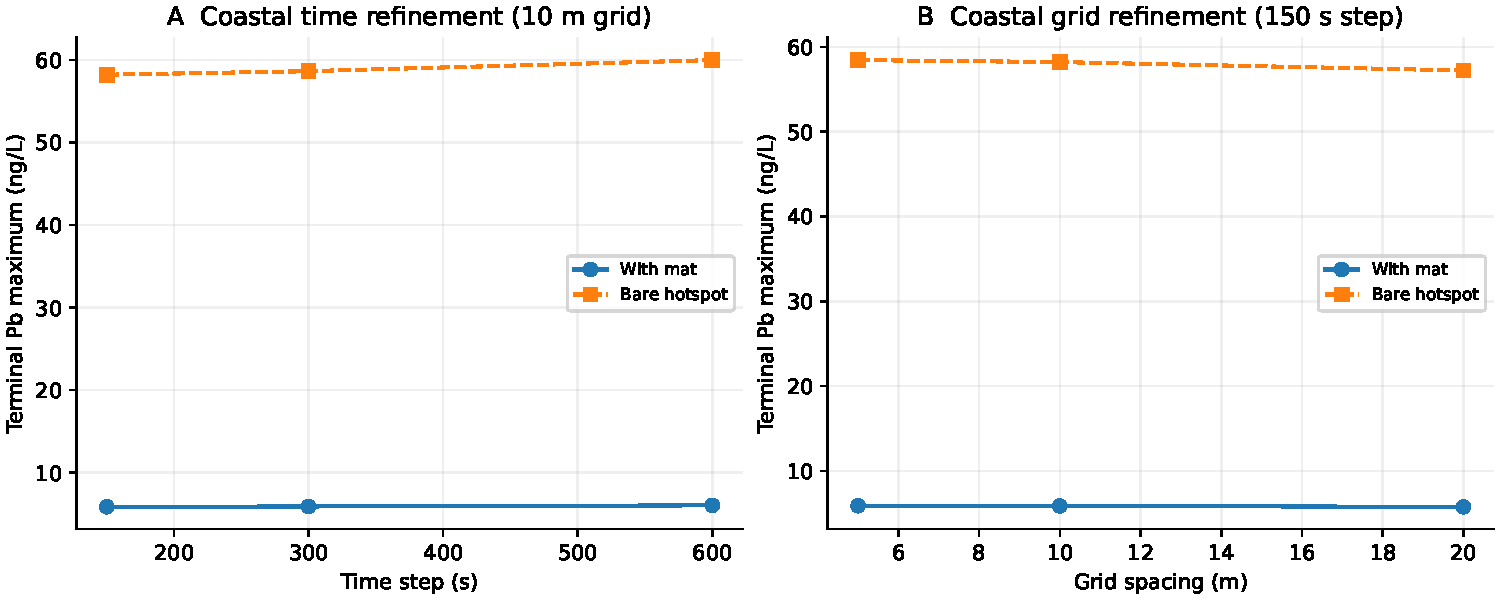
\includegraphics[width=\linewidth]{figures/coastal_discretisation_audit.pdf}
\caption{Coastal numerical sensitivity at a fixed one-year mat state and fixed 24-hour tidal window. Left: time-step refinement on the 10-m grid; right: grid refinement at 150 s. The relative with/bare source response may be more stable than either absolute terminal maximum.}\label{fig:coastal-discretisation-audit}\end{figure}


\section{Deployment scale, targeting and practical evidence requirements}
\label{sec:deployment}

\subsection{Area and material demand}

The deployment calculations are an independent scaling exercise. They do not identify a measured metal hotspot at a munitions site, simulate warfare-agent removal, or establish feasibility of placing a retrievable mat there. The historical dumped-munitions context is documented by HELCOM; the present calculations use selected repository areas to compare square-metre performance with the much larger area potentially requiring intervention.\cite{helcom2025}

For covered area $A$, sorbent loading $L_s$, material price $c_A$ and assumed laying rate $r_A$,
\begin{equation}
M_s=AL_s,\qquad C_{\mathrm{material}}=Ac_A,\qquad
T_{\mathrm{vessel}}=A/r_A.
\end{equation}
The default scenario uses $L_s=4$ kg\,m$^{-2}$, $c_A=240$ EUR\,m$^{-2}$ and $r_A=20{,}000$ m$^2$ per vessel day. The last quantity is an optimistic illustrative production rate, not contractor evidence. Bornholm's primary dumpsite is represented by a published circular radius of three nautical miles.\cite{bornholm2010} With one nautical mile equal to 1,852 m, this gives $\pi(3\times1852)^2=96.9783$ km$^2$. The extended Bornholm area and the Gotland and Skagerrak areas are approximate scale inputs, not newly measured contaminated footprints.

\begin{table}[htbp]
\centering\small
\caption{Area-covering arithmetic recalculated from the deployment module. Costs are material only, and all loading, price and production-rate values are assumptions. Larger areas do not establish contaminant density or treatment suitability.}
\label{tab:deployment-scale}
\begin{tabular}{lrrrr}
\toprule
Area & km$^2$ & Sorbent (t) & Material (EUR bn) & Vessel days \\
\midrule
Synthetic hotspot & 0.0064 & 25.6 & 0.001536 & 0.32 \\
Bornholm primary & 96.978 & 387,913 & 23.275 & 4,849 \\
Bornholm extended & 1,000 & 4,000,000 & 240 & 50,000 \\
Gotland illustrative area & 1,500 & 6,000,000 & 360 & 75,000 \\
Skagerrak illustrative areas & 1,300 & 5,200,000 & 312 & 65,000 \\
\bottomrule
\end{tabular}
\end{table}

The Bornholm primary footprint is approximately 15,153 times the demonstrator's 6,400 m$^2$ hotspot. Its assumed laying requirement is 13.28 years of continuous operation for one vessel at the stated rate, before weather downtime, mobilisation, surveys, anchor placement or retrieval. Figure~\ref{fig:scale} presents these contrasting area scales. The arithmetic is sufficient to show that whole-area coverage is an implausibly large extrapolation of this demonstrator; it is not an economic optimisation or a demonstrated schedule.

The repository also divides sorbent demand by a reference annual global greasy-wool production of 1.76 million tonnes. On that stipulated denominator the primary Bornholm area consumes 22.0\%, and the three larger areas consume 227\%, 341\% and 295\%, respectively. That comparison should be treated as a repository benchmark with uncertain external provenance, rather than an independently established contemporary supply estimate. Greasy wool is not interchangeable with deployable functionalised keratin: extraction yield, processing losses, competing uses, quality selection and fabrication capacity are absent. The comparison therefore cannot establish the actual share of industrial feedstock required.

At EUR 240\,m$^{-2}$, material budgets of EUR 1, 5, 20 and 100 million buy 0.417, 2.083, 8.333 and 41.667 ha, respectively. A suggested 1--2 ha pilot would require 40--80 tonnes of core and EUR 2.4--4.8 million of material before other costs. Its nominal area represents only 0.010--0.021\% of the primary Bornholm circle. This is a scale-limited pilot concept, not a demonstrated feasible first deployment. The calculations omit commissioning, permission processes, vessel capability at depth, monitoring, biological impacts, long-term retrieval and waste treatment.

\subsection{Illustrative receptor-based priority}

The targeting module ranks four illustrative candidate types by proximity to named receptor classes. It evaluates
\begin{equation}
P_j=\sum_{r\in\mathcal R_j}\frac{w_r}{1+d_{jr}/d_{1/2}},
\qquad d_{1/2}=5\ \mathrm{km}.
\label{eq:priority}
\end{equation}
Weights are 1.0 for bathing water, shellfish/aquaculture and water intakes; 0.8 for commercial fisheries; 0.7 for protected habitats; and 0.4 for ports/navigation. Distances and weights are illustrative judgements. Neither depth nor contaminant inventory appears in Eq.~\eqref{eq:priority}; depth is reported alongside the score but does not mathematically penalise it. The score also omits current direction, residence time, exposure duration, receptor population, dose--response and regulatory thresholds.

\begin{table}[htbp]
\centering\small
\caption{Recomputed candidate scores. Chemistry compatibility is a separate label based on listed contaminants, not proof of sorption or complete treatment. Candidate areas and distances are illustrative.}
\label{tab:priority}
\begin{tabular}{p{0.39\linewidth}rrp{0.25\linewidth}}
\toprule
Candidate & Score & Depth (m) & Model-chemistry overlap \\
\midrule
Generic industrial harbour & 2.392 & 8 & Pb, Hg and Cu listed \\
Kolberger Heide, Kiel Bay & 2.161 & 12 & Metal fraction only \\
Bay of L\"ubeck coastal areas & 2.078 & 20 & No energetics model \\
Bornholm primary & 0.375 & 90 & Metal fraction only \\
\bottomrule
\end{tabular}
\end{table}

The harbour example scores 6.37 times the offshore Bornholm example, because of its prescribed receptor set and shorter distances. Figure~\ref{fig:priority} shows this ranking. It supports the proposition that a small intervention should be evaluated against a specific exposure pathway, but it does not prove that these actual sites have this ordering of risk or benefit. More listed receptors increase the score, so completeness of the receptor inventory is itself a source of ranking bias. A real comparison would require a consistent receptor register, spatially resolved benthic fluxes and transport connectivity, followed by an explicit uncertainty and sensitivity analysis.

Contaminant matching is more fundamental than the score. The reviewed Bay of L\"ubeck study documents energetic compounds in water and biota before remediation.\cite{bayLuebeck2025} The present physical model contains Pb, Hg and Cu only. It includes no adsorption, transformation, toxicity or treatment result for TNT, RDX, DNT, arsenic or chemical warfare agents. The manuscript therefore cannot infer suitability for those contaminants from the presence of keratin thiols or a high receptor-proximity score. Activated-carbon/keratin combinations are possible future design questions; they would be different media requiring their own experiments and models.

The repository's recovery comparison, $300{,}000/(2\times365.25)=410.7$ years, is arithmetic for a stipulated 300,000-tonne inventory and a constant two-tonne-per-day operation. It is not a forecast of a national recovery programme: parallel operations, changing technology, prioritisation, weather, object classification and capacity growth are excluded. Neither this extrapolation nor material-only budget coverage demonstrates that capping should replace physical recovery. Both simply illustrate the need to define a bounded, technically suitable intervention.

\subsection{Practical monitoring chain and minimum evidence}

The repository's supplier document is a dated research shortlist rather than a procurement result. It distinguishes contextual sonde candidates (nke and Aqualabo), current meters (Nortek), a historically documented Pb voltammetric system (IDRONAUT VIP), and separate laboratory or topside Hg analysers (P S Analytical). It does not establish stock, current support, a common trace-metal fraction, verified analytical limits in the intended seawater matrix or installed cost. In particular, environmental sondes do not become Pb/Hg analysers by inclusion in a digital monitoring chain.

A practical ingestion architecture would connect a validated digital instrument to a logger or surface gateway and then to the common timestamped record format. Physical serial links such as RS485, RS422 and RS232 are distinct from application protocols and cloud interfaces. The proposed CSV or serial-file replay is an implemented software demonstration route; a generic Modbus emulator cannot establish compatibility with an undocumented manufacturer's register map. Appropriate marine depth rating, pressure, salinity, fouling control, calibration, cycle time, data export and servicing intervals would have to be demonstrated for the selected hardware.

The decisive evidence gap is spatially resolved, contaminant-specific benthic flux at a suitable authorised hotspot. Strong spatial concentration of flux could make a small treated area consequential; uniform flux would make the same intervention proportionately small. No such spatial validation dataset is supplied by the repository. A pilot claim therefore requires, in order, evidence of the target fraction and exposure pathway; a measured site map of source flux and physical seabed conditions; seawater commissioning data on the actual medium; survivability and recovery trials for the assembled mat; and a monitoring design capable of distinguishing sorption, source changes, burial and physical damage. The model organises these questions and exposes the scale problem, but its synthetic results do not answer them experimentally.

\begin{figure}[htbp]\centering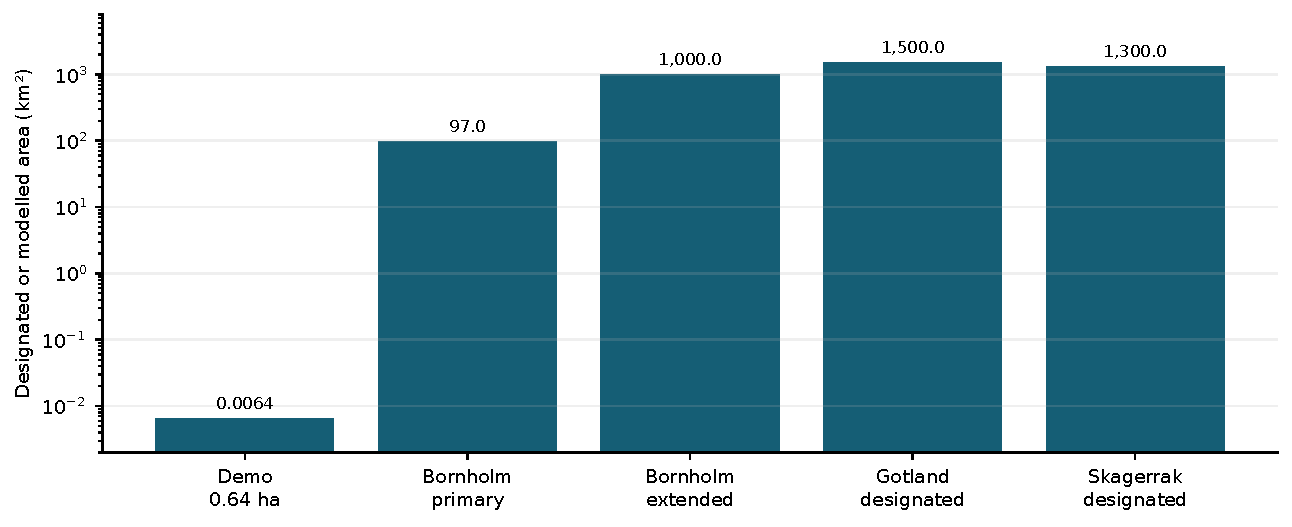
\includegraphics[width=\linewidth]{figures/scale.pdf}
\caption{Area comparison redrawn from the regenerated gallery data. The four regional areas are designated historical dumping areas with different definitions; they are neither mapped continuous contamination nor eligible mat footprints. The hypothetical 0.64~ha hotspot is orders of magnitude smaller. The logarithmic axis makes this scale gap visible.}\label{fig:scale}\end{figure}
\begin{figure}[htbp]\centering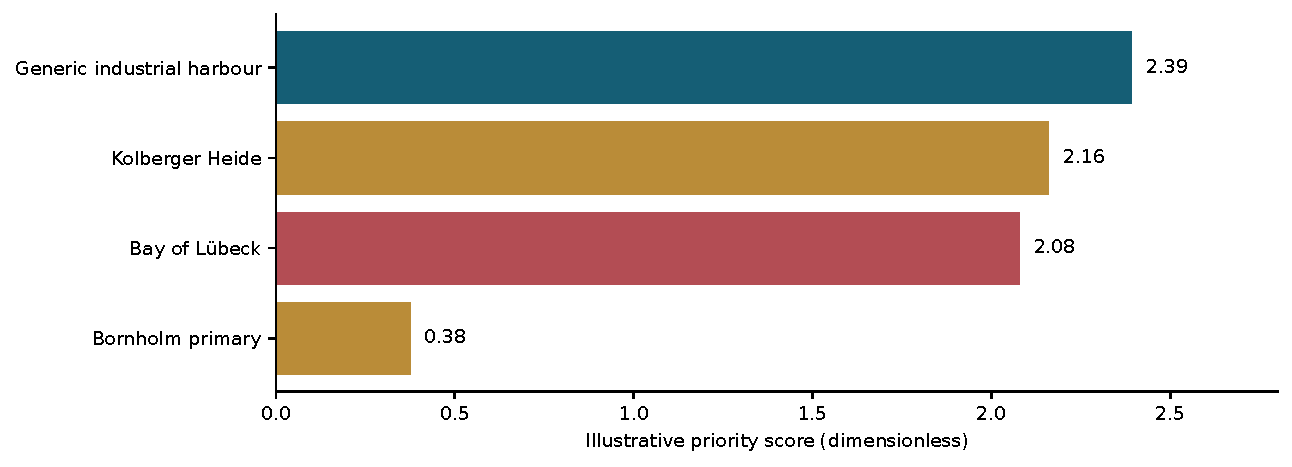
\includegraphics[width=\linewidth]{figures/priority.pdf}
\caption{Illustrative candidate scores reproduced from the repository's deterministic priority function. The generic harbour has the strongest assumed match to the modelled metal chemistry. Scores use assumed receptor distances and weights; depth and logistics do not enter the score. The ordering is not a measured risk ranking or site-selection decision.}\label{fig:priority}\end{figure}
\begin{figure}[htbp]\centering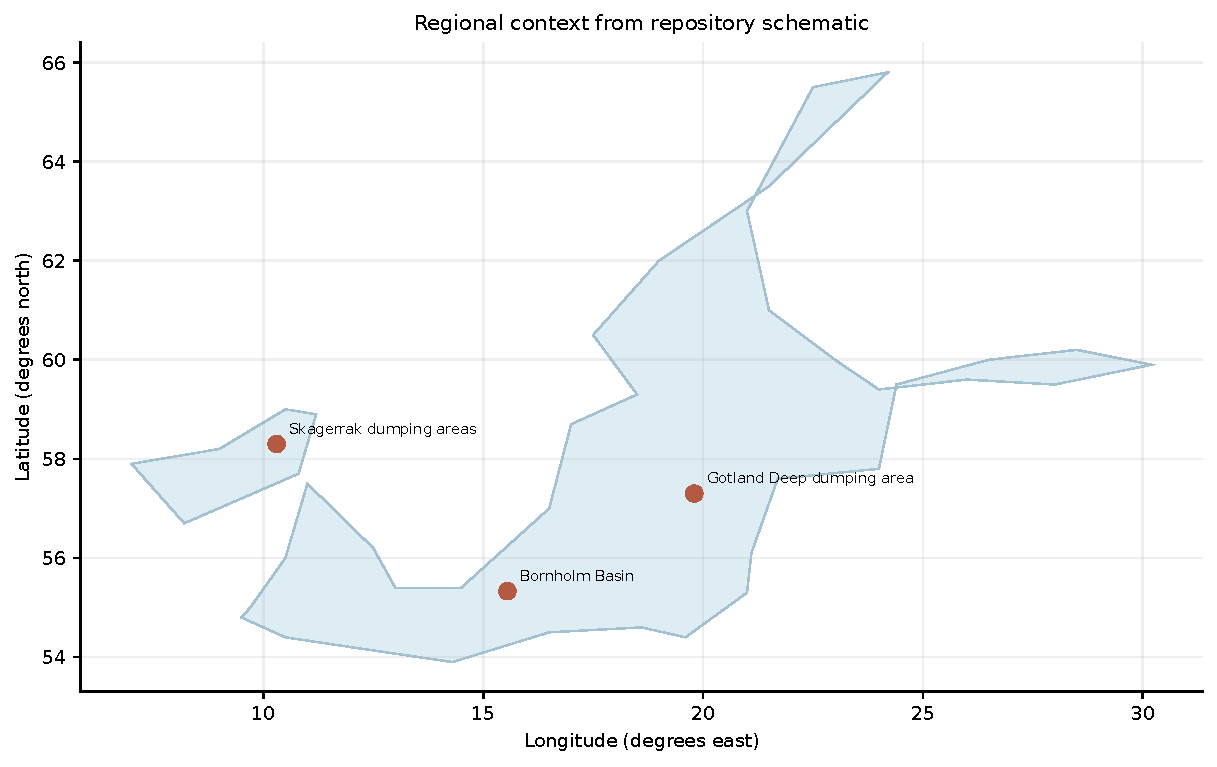
\includegraphics[width=.94\linewidth]{figures/context.pdf}
\caption{Regional context redrawn from the repository's schematic coordinates. The outline is deliberately schematic and is not a navigational or survey map. Markers provide geographical context for the scale calculation; no mat deployment, object location or handling operation is implied.}\label{fig:context}\end{figure}
\clearpage
\section{Discussion and conclusions}
\label{sec:discussion}
\subsection{What the revised simulations establish}
The revised implementation separates whole-hotspot emission, column resistance, chemical storage and the evidence available to an operator. Consistent tile geometry now gives the configured footprint, damage changes the corresponding source cells, and the timeline and spatial source share the same area weighting. Exact initial and final times, event boundaries and frozen-state plume diagnostics remove the previous age offset. These changes materially alter the deployment interpretation of the earlier plots.

High attenuation does not establish high recovery. Physical resistance persists when chemical storage changes little, and nominal capacity may remain unused because accessibility and equilibrium partitioning limit uptake. The numerical studies quantify discretisation effects; they do not make the assumed material parameters measured properties. The corrected barrier reference uses the same discrete stationary operator, avoiding a small spurious chemistry increment from comparing different boundary discretisations.

Material scale remains direct arithmetic: at 4~kg\,m$^{-2}$, every hectare requires 40~t of core. Whether a small treated area could reduce a large share of exposure depends on measured source heterogeneity and receptor connectivity, neither of which the default uniform hotspot supplies.

\subsection{Interpreting bumps and non-monotone plots}
The revised plots preserve discontinuities at prescribed source changes, physical damage and accepted replacement. Before and after states at the same event time are connected vertically. These are consequences of explicit scenario interventions. A source decrease can also lower the attenuation ratio temporarily because stored contaminant and porewater respond on a finite time scale while the bare-reference denominator changes immediately. Such a response need not indicate negative capture or a failed integrator.

The actual source increase in scenario C illustrates the denominator effect in the opposite direction: at year 2, Pb attenuation rises from 82.72\% to 85.08\% while absolute residual emission also rises. The bare-reference flux increases faster than the residual flux at that instant. The subsequent sharper attenuation decline near years 2.2--2.25 coincides with the Pb capacity ceiling being reached, without a service event. In scenario D, displacement at year 1.5 lowers Pb attenuation by 9.55 percentage points. The lost-tile survey arrives later, and replacement on day 750 raises it by 10.89 points while lowering average active-media saturation. A separate local-damage event at year 2.2 lowers attenuation by 3.17 points. Its subsequent punctured survey class does not satisfy the strict integrity-upper-bound replacement threshold, so that damage does not produce a second service. These timings reflect the specified events, survey cadence and policy rules.

Coastal endpoint maxima vary with the duration and tidal phase of the plume window. A 24-hour window is not an integer number of the prescribed M2 cycles. Its final spatial maximum is a phase-dependent statistic, not a monotonic steady-state convergence measure. The same-phase and numerical-resolution studies separate these effects. Maps are displayed with their actual mat age and matched with/without concentration scales; all time curves include the full reported range.

Some sharp responses arise from constitutive assumptions that remain unvalidated. In particular, exactly capacity-locked cells do not desorb in the implemented law, whereas a just-unsaturated cell can respond to flushing. The independent clean-water comparison exposes this discontinuity. It is retained explicitly for this demonstrator, and should be revisited before using the model to predict remobilisation or service life.

\subsection{Limits of the accounting and monitoring models}
The full-footprint reactive-column ledger closes for the numerical column problem and records active and retrieved inventories separately. Whole-hotspot emission includes bypass and changing effective area. These two diagnostics do not constitute a closed, fully coupled sediment--mat--water inventory when bypass or damage changes: the column inventory is not scaled by the bypassed fraction, and no finite sediment reservoir is resolved. Attenuation against a hypothetical bare reference is therefore not synonymous with contaminant recovered in keratin.

The columns use a clean overlying-water boundary over the long timeline; episodic plume windows start clean, hold the source fixed, and do not feed concentrations back into the earlier column history. The two-dimensional model prescribes currents and mixing rather than solving hydrodynamic momentum. These are explicit reduced-model assumptions. A field assessment would need transport connectivity, heterogeneous seepage, realistic boundaries and appropriately coupled budgets.

The observation clock now spans the experiment, campaign draws are independent of the decision partition, analytical fractions are matched, and quality-control flags affect the controller. Zero burial and missing Cu no longer create positive evidence of a failure. Observations from retired media and exposure windows crossing replacement are excluded from current-media estimates. Nevertheless, the instrument layout remains sparse, uncertainty intervals are heuristic rather than coverage-calibrated probabilities, and recommendations for additional sampling do not yet alter the sample programme. A zero-service outcome cannot by itself prove that a mat was healthy or that monitoring saved a lifecycle cost.

The coupled treatment of censoring is also incomplete. Although the data contract preserves non-detect and above-range bounds and the standalone estimator can propagate them, the current scalar QC has no applicable interval check for the generated censored records. It marks them not evaluated, and the passed-only estimation gate excludes them. Scenario A therefore lacks usable Hg chamber evidence throughout its one-year run even though two bounded Hg chamber results have arrived. This conservative information loss helps explain repeated sampling requests; it does not establish absent Hg flux or validated use of non-detect evidence. In scenarios B and C, later quantified chemistry is available, but wide saturation intervals evaluated at their midpoint remain below the replacement trigger. The fully saturated physical Pb state in scenario C is not directly visible to the policy.

\subsection{Material evidence and priorities for experiments}
The supplied papers support keratin as a candidate sorbent and provide numerical laboratory observations. They do not identify a seawater-qualified finished wool/feather core. The reviewed high mercury uptake concerns chemically modified human hair; the high multi-metal removal concerns a keratin--graphene-oxide composite. Batch removal percentage, uptake at one initial concentration and fitted maximum capacity are different quantities. This report preserves those distinctions and retains the demonstration's operating parameters as assumptions.

A useful experimental sequence should test the finished core in representative seawater and porewater, with dry loading, pH, salinity, sulphide, organic matter and metal fractions measured. Batch uptake should be complemented by flow-through breakthrough, desorption, mixed-ion competition and ageing. Empty geotextile and inert-core controls are needed to separate resistance from chemical capture, and an alternative sorbent can test whether keratin adds a practical advantage.

Ecological assessment must include fibre and particle release, degradation products, effects on benthic exchange and potential methylmercury production. The model contains no microbial Hg transformation or verified ecological benefit. Any later pilot should address a characterised authorised source and measurable flux or exposure endpoints, with retrieval and disposal designed alongside installation.

\subsection{Conclusions}
The revised repository provides reproducible synthetic scenarios, consistent spatial and temporal reporting, a documented numerical audit, and a traceable distinction between published material evidence and assumed operating settings. The plot anomalies included both correct responses to interventions or tides and implementation defects; the identified integration and reporting defects have been corrected and the affected results regenerated. The remaining limitations concern material calibration, constitutive choices, coupling, sparse evidence, censoring-aware QC and deployment feasibility. The defensible use is hypothesis testing and experimental design, with field efficacy and reliable servicing advantage still to be established.

\clearpage
\phantomsection
\addcontentsline{toc}{section}{References}
\bibliographystyle{unsrtnat}
\bibliography{references}
\clearpage
\appendix
\section{Reproduction and numerical traceability}
\label{app:reproduction}
The manuscript resides in the repository's \path{manuscript/} directory together with its section sources, BibTeX database, vector figures, portable result summaries and verification records. The full interactive gallery is \path{docs/gallery/index.html}. The provenance inventory lists content hashes and the source revision used for the corrected simulations. Internal development prompts and third-party article PDFs are not distributed as manuscript source evidence.

\subsection{Build the manuscript}
From \path{manuscript/}, use the included PowerShell build script or run:
\begin{verbatim}
pdflatex -interaction=nonstopmode -halt-on-error manuscript.tex
bibtex manuscript
pdflatex -interaction=nonstopmode -halt-on-error manuscript.tex
pdflatex -interaction=nonstopmode -halt-on-error manuscript.tex
\end{verbatim}
All required images and bibliography data are local. The source includes a compatibility patch for the installed longtable version; it is a no-op where the upstream correction is already present.

\subsection{Recompute the scientific results}
Install the repository's declared Python dependencies in a separate environment. From the repository root, run:
\begin{verbatim}
python -m pytest -q
python tools/build_gallery.py --workers 2
python tools/revision_numerics.py
python tools/benchmark_layer_memo.py --days 30
python tools/timescale_check.py --workers 2
python tools/export_manuscript_data.py
python manuscript/extract_gallery.py
python manuscript/make_figures.py
python tools/render_manuscript_tables.py
python tools/render_numerical_results.py --output manuscript
\end{verbatim}
The gallery and time-scale tools cache their own local computations using source/configuration fingerprints. Locally produced pickle caches are not portable evidence and must not be loaded from untrusted sources. Portable JSON summaries, configuration hashes and rendered figures are committed. Complete per-run exports in \path{results/revision/} include observations, estimate histories, actions, ledgers, configurations and offline reports and can be regenerated using the commands above.

The verification records cover the entire test suite, all regenerated scenario and policy ledgers, source-map/timeline agreement, exact horizons, observation identifiers, numerical refinement, and PDF build checks. Passing these checks establishes the stated implementation behaviour, not empirical validation of seawater capacities or ecological outcomes. Table values retain a useful reporting precision without implying comparable physical certainty.

\section{Supplier and external-data evidence catalogue}
\label{app:suppliers-data}

\subsection{Instrument and service candidates}

The repository's scientific sensor matrix records nineteen candidates as of 8 September 2026. Table~\ref{tab:suppliers} summarises that dated inventory, including its gaps, rather than asserting present availability or independent performance verification. All interface descriptions in the table are \emph{reported by that inventory}; hardware revisions, manuals, calibration and suitability for a particular seawater deployment remain to be confirmed. No instruments were connected or field-tested, and no supplier quotations support the model's costs. The separate summary also mentions WiMo sensors and a possible PSA 10.226 topside Hg analyser.\cite{repository}

\begingroup\small
\setlength{\tabcolsep}{4pt}
\begin{longtable}{p{0.28\linewidth}p{0.22\linewidth}p{0.43\linewidth}}
\caption{Complete grouped supplier inventory. L: a listing recorded in the repository; H: historical evidence; I: indexed lead with incomplete direct retrieval; R: research prototype. These are source-record statuses, not current stock or suitability certifications. FR, IT, DK and NL identify EU-based suppliers; the remaining countries listed are European non-EU locations.}\label{tab:suppliers}\\
\toprule
Supplier and candidate & Purpose; recorded interface & Status and unresolved point \\
\midrule
\endfirsthead
\toprule
Supplier and candidate & Purpose; recorded interface & Status and unresolved point \\
\midrule
\endhead
\bottomrule
\endfoot
Nortek, Norway: Aquadopp 500 m Gen 2 & Point current; RS422, vendor configuration software & L. Current context only; duty cycle and exact binary integration need confirmation. \\
Sonardyne, UK: Origin 65 ADCP & Current profile; RS232, Ethernet, acoustic link, portal/SDK & L. Deep-profile instrument; useful near-bed resolution in the shallow model domain is unestablished. \\
Aanderaa, Norway: DCPS 5400/DCS family & Currents; serial or AiCaP bus, model dependent & L. Exact model accuracy, outputs and support must be established from its manual. \\
Star-Oddi, Iceland: DST centi-TD & Temperature/depth; recovered logger with PC/SeaStar readout & L. Data become available on retrieval; this is not a telemetered chemistry channel. \\
Aqualabo, FR: CTZN & Conductivity, salinity, temperature; Modbus over RS485 or SDI-12 & L. Register map and deployment depth unresolved; IP68 alone is insufficient. \\
Aqualabo, FR: PHEHT & pH/redox/temperature; Modbus/SDI-12 reported & L. Some interface details came from third-party listings; seawater calibration and drift unresolved. \\
Aqualabo, FR: NTU & Turbidity; Modbus over RS485 or SDI-12 & L. Depth, fouling control and matrix response need confirmation. \\
nke, FR: MoSens; WiMo family & Context carrier/sonde; Modbus, configuration tools & L. Electrical layer and exact registers depend on selected sensors; no demonstrated open API. \\
IDRONAUT, IT: VIP & Dynamic/labile Pb, Cd, Cu, Zn; historical RS232/software & H. Current support and seawater limits not verified. A mercury electrode does not imply an Hg analyte channel. \\
Metrohm, Switzerland: 884 Professional VA, Bi electrode & Laboratory Pb/Cd; viva software/PC & L. Cited application method lacks a demonstrated spiked-seawater Pb result; field deployment not applicable. \\
Milestone, IT: DMA-80 evo & Laboratory total Hg, possible media assay; PC export unresolved & I. Mass sensitivity does not establish a seawater concentration limit; species-specific Hg unresolved. \\
P S Analytical, UK: 10.035 Merlin; 10.226 lead & Laboratory total Hg; possible topside liquid analyser & I. Water handling, fraction, saline-matrix limits and data outputs not verified in the repository. \\
DGT Research, UK: LSPM-NP & Sediment accumulated labile metals; passive, no digital interface & L. Retrieval and laboratory analysis required. Listed Chelex device does not establish Hg suitability. \\
Unisense, DK: MiniChamber Lander & Chamber incubation; logger, RS232 guest devices & L. Listed sensors are not Pb/Hg detectors; timed water subsampling and metal analysis need validation. \\
Rhizosphere Research Products, NL: Rhizon CSS & Porewater extraction; passive vacuum sampler & L. No direct measurement or telemetry; metal blanks, adsorption and in-mat sampling need evaluation. \\
Exail, FR: Gaps M5 USBL & Acoustic position; output format unresolved & L. Headline slant-range accuracy does not establish practical tile-displacement precision. \\
Blueye, Norway: X3 & ROV imagery/condition; payload ports, app and SDK & L. Visible condition only; buried material and chemical loading remain unobserved. \\
Subsea Tech, FR: inspection/survey services & ROV/USV survey, photogrammetry, bathymetry & L. No sediment-cap project validation, availability or quoted service rate established. \\
University of Geneva, Switzerland: TracMetal/Au-GIME & Research in-situ Hg(II) and other metals; protocol unresolved & R. Research evidence does not establish a supported purchasable system or a multi-year deployment. \\
\end{longtable}
\endgroup

The proposed pilot architecture combines current/context measurements, passive Pb exposure, porewater grabs, chamber subsamples and physical surveys, followed by an assay whenever media are retrieved. The repository has not verified a commercially supported instrument providing the simulated six-hourly Pb channel at its assumed 12 ng\,L$^{-1}$ detection limit. It has also not verified an equivalent continuous in-situ Hg channel. These are findings about the documented search, not claims that no such technologies can exist.

A control area is essential to interpreting attenuation against a changing source: matching chamber and porewater measurements over capped and uncapped patches would support a counterfactual comparison, with uncertainty from spatial variability. Clean sampling, preservation, matrix-specific analysis and analytical fraction must accompany the instrument choice; established water-analysis methods do not make the complete proposed seabed system validated.\cite{epa1631,epa2008} Media capacity in place, internal fouling, edge bypass, methylmercury formation and benthic-community response remain beyond this inventory's demonstrated observations.

\subsection{Scientific data catalogue and access state}

The data catalogue contains eight resources and two explicit search gaps. None of its external datasets is bundled or used to calibrate the default simulations. Its access labels distinguish a checked portal, a discovered listing, and a retrieved metadata record; none alone proves that a numerical dataset was downloaded and incorporated. The packaged synthetic observation file is a format/edge-case fixture, not a measured time series or a sorption-calibration dataset.\cite{repository}

\begin{table}[htbp]
\centering\small
\setlength{\tabcolsep}{4pt}
\caption{Scientific resources recorded by the repository and their actual role. External numerical data were not loaded into the default report scenarios.}
\label{tab:datasets}
\begin{tabular}{p{0.26\linewidth}p{0.34\linewidth}p{0.33\linewidth}}
\toprule
Resource & Potential scientific contribution & Repository access/integration state \\
\midrule
ICES DOME (D1) & Contaminants/effects in sediment, water and biota; European monitoring context & Portal confirmed; no dataset download or model fit.\cite{icesDome} \\
OSPAR CEMP 2024 (D2) & Assessed hazardous-substance levels and trends & Dataset listing recorded; not downloaded. \\
OSPAR ODIMS (D3) & Environmental datastream catalogue & Portal confirmed; no model integration. \\
EMODnet Chemistry (D4) & Aggregated European-seas contaminant observations/products & Portal confirmed; not a source of default hotspot concentrations.\cite{emodnetChemistry} \\
HELCOM metals indicators (D5) & Baltic status and trends & Indicator/portal context; not a local porewater calibration.\cite{helcomMercury} \\
Hyl\'en et al., Baltic benthic fluxes (D6) & Chamber-data structure: 498 phosphorus fluxes, 59 stations & Record retrieved; phosphorus only, not Pb/Hg validation.\cite{hylen2025} \\
US EPA sediment amendments (D7) & Treatment-practice and performance context & Technical-report listing; not a calibration dataset. \\
USGS benthic chamber (D8) & Chamber design and measurement method & Method reference; shallow freshwater setting.\cite{benthicFluxMonitoring} \\
\bottomrule
\end{tabular}
\end{table}

ICES/EMODnet sediment concentrations cannot be inserted into the porewater boundary condition by changing units: solid-to-water partitioning requires additional evidence and uncertainty. The recorded gaps are an open dataset of marine reactive-cap Pb/Hg flux attenuation and isotherms for the actual keratin core in seawater. ``Not found in the repository's search'' is the supported conclusion, rather than a universal assertion of absence. Product-specific attribution, access terms, redistribution permissions, analytical fractions and update dates would need checking before any new dataset is incorporated.

\subsection{Supplied laboratory literature and parameter records}

The paper audit adds three fully inspected articles: the 35-page Enkhzaya journal pre-proof, the 14-page Zubair composite article and the 14-page Zubair review \citep{enkhzaya2020,zubair2025,zubair2026}. Page numbers in the companion traceability register refer to those supplied copies. Enkhzaya's Cu isotherm parameters are on PDF page~32 (printed page~31), kinetic parameters on PDF page~33, and experimental conditions on pages~5 and~21. Zubair's Pb composite result appears in the abstract and Fig.~10, with matrix, dose and preparation details on page~13. The review's modified-human-hair Hg lead appears on page~5 and was checked against the primary publisher abstract/highlights \citep{liang2023}; the full Hg methods were not retrieved.

The source register distinguishes a fitted maximum, a dose-dependent batch uptake, removal efficiency, a distribution ratio and a kinetic coefficient. It stores original units, derived conversions, source discrepancies and whether a number entered the operating configuration. None of the newly extracted numbers was substituted into the default seawater model. The previously cited review supplied background context; the numerical defaults and synthetic commissioning ranges retain their assumption labels. Article hashes permit exact-copy identification, while the supplied PDFs and article images are not redistributed. Section~\ref{sec:paper-traceability} explains the resulting corrections and transfer limits.

\subsection{Geographical and current-data adapters}

The geodata module exposes three distinct capabilities: synthetic forcing, a cached map with illustrative physics, and import of a locally cached current product. The normal scenario runner uses the prescribed forcing directly. Its outputs do not become observed geography, measured metal fields or external-current simulations because these adapters exist. Copernicus Marine is a candidate provider of resolved current products; its documented IBI product is contextual rather than data used in these default runs.\cite{copernicusIbi}

An imported cache is a project JSON representation containing coordinate arrays, two velocity fields and metadata for product identity, version, source depth, native resolution, temporal averaging, tide resolution, citation and licence. It is not a direct download client for arbitrary Copernicus or EMODnet products. Missing files are refused. The caller must already project coordinates into the metric computational system; the adapter uses nearest-neighbour regridding, and no finer grid creates new sub-grid information. Bathymetry remains visual context in this build, not a spatially varying numerical water depth or a hydrodynamic solver.

The current cache contains one pair of two-dimensional velocity arrays, without a time dimension. Repeated calls timestamp the same fields; a metadata declaration of tide resolution does not itself provide evolving tidal currents. The adapter rejects a declared non-tide-resolving product when requested for a tidal scenario, but a genuine temporal import and coupling still require additional implementation and verification. Thus external-data pathways are defined software interfaces and evidence requirements, while the manuscript's scenario results remain offline synthetic demonstrations.

\clearpage
\section{Additional spatial figures}
\label{app:spatial}
These plates complete the six-scenario comparison. The principal late comparison uses a three-year state where that age exists, and the actual one-year endpoint for scenario A. The different age also gives A a different prescribed tidal phase, which explains its different plume direction. The final-age source plate also shows all actual scenario endpoints. With/without concentrations share a scale within each pair. A zero source outside the prescribed hotspot means no modelled input, not a measurement below detection.

\figpage{flux_00}{Initial residual Pb source from the unadvanced commissioned mat state. The mat core begins with zero contaminant inventory; uncovered area and edge bypass still emit.}{fig:fluxzero}
\figpage{flux_final}{Residual Pb source at each scenario's actual final age, shown in each panel. Baseline coverage is 100\% and scenario F coverage is 45\% before degradation/bypass.}{fig:fluxfinal}
\figpage{spatial_A}{Scenario A at its actual one-year endpoint: water concentrations, concentration ratio and effective cover.}{fig:spatialA}
\figpage{spatial_C}{Scenario C at three years, after the prescribed source increase. Larger concentrations reflect both stronger driving and the mat response.}{fig:spatialC}
\figpage{spatial_D}{Scenario D at three years. Fault targets now overlap the source, and snapshots use the condition and replacement history at this age.}{fig:spatialD}
\figpage{spatial_E}{Scenario E at three years. Delayed observations alter evidence availability; physical changes occur only through accepted service events.}{fig:spatialE}
\figpage{spatial_F}{Scenario F at three years. A thin core, 45\% geometric coverage, increased seepage and larger edge leakage form a compound stress case.}{fig:spatialF}
\clearpage
\section{Assumption coverage and remaining evidence gaps}
\label{app:assumptions}
The report's numerical tables state the current implemented defaults. This final register groups the assumptions that are not well represented by a single scalar or that could otherwise be lost among implementation details.
\begin{longtable}{p{.24\linewidth}p{.64\linewidth}}
\caption{Qualitative assumption register and scientific implications.}\label{tab:assumption-register}\\
\toprule Assumption family & Scope and consequence\\\midrule\endfirsthead
\toprule Assumption family & Scope and consequence\\\midrule\endhead
Sediment source & Concentrations and seepage are prescribed piecewise constants over a hypothetical uniform hotspot. No finite sediment reservoir, source depletion, heterogeneous redirection, consolidation or bioturbation is resolved.\\
Material selectivity & Element-specific availability and allocations are fixed assumptions. Independent capped uptake laws do not represent a coupled competitive multispecies sorption model.\\
Chemical species & Pb, Hg and Cu physical channels are element-level abstractions. No mechanistic equilibrium speciation, microbial transformation or methylmercury production is solved.\\
Medium ageing & Fouling modifies assigned transport/reaction properties; capacity loss, damage, displacement and burial are distinct state mechanisms. Real biological degradation, particle release and structural fatigue are not calibrated.\\
Textile physics & Carrier layers contribute diffusive resistance with assumed geometry and porosity. Full pressure-driven geotextile hydraulics, strain and anchoring mechanics are absent.\\
Hydrodynamics & Uniform prescribed tidal velocity replaces a momentum model; mixing depth and horizontal diffusivity are constant. Boundary water is clean, exported contaminant does not re-enter, and vertical structure is unresolved.\\
Coupling & Multi-year columns see zero bottom-water concentration. Plume windows start clean and use frozen sources. They do not represent a continuous multiyear coastal concentration history.\\
Observation synthesis & Noise, missingness, analytical limits, delays and campaign timing are assumed. Instrument names in the research inventory do not validate those values or imply a live connection.\\
Uncertainty & Reported intervals use deterministic arithmetic and assumed widening. Material ranges are not joint probability distributions; ensemble and nominal confidence labels do not establish calibrated predictive coverage.\\
Maintenance & Rules use thresholds and attribution heuristics. Simulated acceptance of replacements is not hardware actuation. The sampling programme does not adapt when further sampling is recommended.\\
Economics & Every quoted euro value is assumed. Service ledgers omit complete installation, monitoring, permitting, retrieval and long-term disposal accounting. Recovered material has no assumed resale credit.\\
Deployment & Designated historical areas, generic receptors and fixed production rates are illustrative. No selected site, feasible laying campaign, technical access or bounded receptor benefit is established.\\
Environmental benefit & Lower modelled dissolved concentration is not a demonstrated reduction in bioavailability, toxicity, methylmercury, benthic harm or human exposure. No field outcome is asserted.\\
Scope of future extensions & Optimisation, formal value-of-information analysis, fitted machine learning and a field-calibrated digital twin are outside the implemented result set.\\
\bottomrule
\end{longtable}

\end{document}
